\documentclass[serif,mathserif]{beamer}  % For use with beamer v 2.20
%\documentclass[handout,serif,mathserif]{beamer}

%% NOTES %%%%%%%%%%%%%%%%%%%%%%%%%%%%%%%%%
\setbeameroption{show only notes} 
\newcommand{\emptynote}{\note{\mbox{}}}
%!TEX root = tutorial01-slidesonly.tex
%!TEX root = tutorial01-splitshow.tex


%%%%%%%%%%%%%%%%%%%%%%%%%%%%%%%%%%%%%%%%%%%%%%%%%%
%% IMPORTANT:
%% IN ORDER NOTES TO WORK WELL YOU HAVE TO ADD A NOTE TO EACH SLIDE!!!!
%% That is, at least a \emptynote command must be added to each slide.
%%%%%%%%%%%%%%%%%%%%%%%%%%%%%%%%%%%%%%%%%%%%%%%%%%


% RANDOM IDEAS:
%
% 1.
% Data: Kepler
% System identification: Newton
% Kepler, Newton, Gauss etc. pioneered machine learning?
% Newton: "Hypotheses non fingo" (I feign no hypotheses) ~ Occam's Razor
%

% Application ideas
% - Reviewing process at journals --> queuing system
% - Active balancing (Shin & Ni)
% - Helicopter landing on a moving deck
% Kitenergy: Tethered aircraft for wind energy generation ("high altitude wind energy")
% -- they use MPC; wind: disturbance, reward: energy generated, + safety guarantees (stay away from the ground); KE-yo-yo prototype; http://www.kitenav.com/; Mario Milanese, ACC Invited Talk


%\transdissolve

%	\setbeamercolor{postit}{fg=black,bg=yellow}
%	\begin{beamercolorbox}[sep=1em,wd=5cm]{postit}
%	Place me somewhere!
%	\end{beamercolorbox}


\usepackage{etex}
\usepackage[absolute,overlay]{textpos}
\usepackage{pdfsync, xspace}
\usepackage{pstricks,pst-node}
\usepackage{multimedia}
\usepackage[normal,tight,center]{subfigure}
\setlength{\subfigcapskip}{-.5em}
\usefonttheme[onlymath]{serif}

\mode<article> % only for the article version
{
  \usepackage{fullpage}
  \usepackage{hyperref}
}



\mode<presentation>
{
%  \setbeamertemplate{background canvas}[vertical shading][bottom=red!10,top=blue!10]
%  \setbeamertemplate{background canvas}
%  \usetheme{CambridgeUS}
  \usetheme{Boadilla}
}

%  There is a VERY rich set of possible
%  styles of presentations and color themes.  See the
%  beamer documentation for a full list of possibilities.
%\usetheme{Warsaw}  % JuanLesPins  Rochester
%\usetheme{JuanLesPins}

           %  Berkeley  Palo Alto    with sidebar and top
           % Goettingen  Marburg     with sidebar
           %  Copenhagen  Luebeck  Warsaw
%\usecolortheme{lily}
%\usecolortheme{default}
%\usecolortheme{crane}
\usecolortheme{beaver}


\usepackage{times}
\usepackage{multicol}
\setbeamercovered{dynamic}

%\usepackage{pgfarrows}
%  Don't need to load the pgf package, but it has
%  has itself some packages you might want, such as
%  pgfarrows,,pgfnodes,pgfautomata,pgfheaps
%  See the pgf documentation.


% \beamertemplatetransparentcovereddynamic
        % overlays that are upcoming are transparent, in
        % a manner that depends upon how far ahead  they are.


% \beamertemplatetransparentcovereddynamic
        % overlays that are upcoming are transparent, in
        % a manner that depends upon how far ahead  they are.

%\usepackage{beamerthemesplit}
%\usepackage{beamerthemebars}
% beamerthemelined
% beamerthemetree
% beamerthemetreebars
% Note: must be compiled with PDFLatex!!

%\usepackage{graphicx}
% support for Hungarian
%\usepackage[magyar]{babel}
%\usepackage[latin2]{inputenc}

%!TEX root = tutorial01-splitshow.tex


\usepackage[textwidth=\marginparwidth]{todonotes}
\usepackage{pdfsync}
\usepackage{hyperref}
\usepackage{fancybox}

% For citations
\newif\ifnumcites
%\numcitestrue
\numcitesfalse




% The paper has an extended (long) version and a short version
\newif\iflong % Sometimes we want to keep two versions; a short and a long one -- this is useful for that..
%\longfalse
\longtrue

% Turn on/off notes and descriptions of research problems
\newif\ifcomm
%\commfalse % also turns off internal todo comments
%\commtrue

% Turn on/off internal todo comments
\newif\iftodo
\todofalse
%\todotrue


\ifnumcites
  \usepackage[numbers]{natbib}
  \bibliographystyle{plainnat}
\else
  \usepackage{natbib}
  \bibliographystyle{apalike}
\fi
%\bibliographystyle{apalike}
% plain, acm, ieeetr, alpha, acm, abbrv, siam
% plainnat.bst, abbrvnat.bst and unsrtnat.bst
% http://web.reed.edu/cis/help/LaTeX/bibtexstyles.html

\if0
\newcommand{\citep}[1]{\cite{#1}}
\newcommand{\citet}[1]{\cite{#1}}
\newcommand{\citealt}[1]{\cite{#1}}
\newcommand{\iftextcite}[1]{}

\newcommand{\npcite}[1]{\cite{#1}}
\newcommand{\yrcite}[1]{\cite{#1}}
\fi



%\usepackage{amsthm}

\usepackage{amssymb}
%\usepackage[dvips]{graphics}
\usepackage{amsmath,amsthm,amsfonts} % Learn about the AMS package, again very useful!

\usepackage{graphicx}
\usepackage{epstopdf}
\usepackage{stmaryrd}
\usepackage{dsfont}
%\usepackage{small-headings}


\newif\ifshort
\iflong
	\shortfalse
\else
	\shorttrue
\fi


% THEOREMS -------------------------------------------------------
\theoremstyle{plain}
\newtheorem{thm}{Theorem}
\newtheorem{cor}[thm]{Corollary}
\newtheorem{lem}[thm]{Lemma}
\newtheorem{prop}[thm]{Proposition}
\newtheorem{conj}[thm]{Conjecture}
\newtheorem{proofthm}{Proof of Theorem 2}

%\renewtheorem{definition}[thm]{Definition}
\theoremstyle{definition}
\newtheorem{defn}{Definition}
%\theoremstyle{remark}


\newtheoremstyle{example}% ?name? 
{3pt}%	?Space above? 
{3pt}%	?Space below? 
{\itshape}%	?Body font?
{}%	?Indent amount?1 
{}% ?Theorem head font? 
{:}%	?Punctuation after theorem head? 
{.5em}%	?Space after theorem head?2 
{}%
\theoremstyle{example}
\newtheorem{ex}{Example}
%\newtheorem{fact}{Fact}
\newtheorem{rem}{Remark}

\newcounter{assumption}%[section]
\newcommand{\theassumptionletter}{A}
\renewcommand{\theassumption}{\theassumptionletter\arabic{assumption}}

\newenvironment{ass}[1][]{\begin{trivlist}\item[] \refstepcounter{assumption}%
 {\bf Assumption\ \theassumption\ #1} }{%\par\nobreak\noindent\sl\ignorespaces}{%
 \ifvmode\smallskip\fi\end{trivlist}}
\newcommand{\aref}[1]{(\ref{#1})}
\newenvironment{ass*}[1][]{\begin{trivlist}\item[] %
 {\bf Assumption\  #1} }{%\par\nobreak\noindent\sl\ignorespaces}{%
 \ifvmode\smallskip\fi\end{trivlist}}


%\newenvironment{remark}
\newtheorem{remark}{Remark}

%\newenvironment{proof}{{\bf Proof.}}{\hfill\rule{2mm}{2mm}\\}

% Keep whatever you need from here


\newcommand{\norm}[1]{\left\Vert#1\right\Vert}
\newcommand{\smallnorm}[1]{\|#1\|}
\newcommand{\abs}[1]{\left\vert#1\right\vert}
\newcommand{\supnorm}[1]{\norm{#1}_\infty}

\newcommand{\set}[1]{\left\{#1\right\}}
\newcommand{\cset}[2]{\left\{\,#1\,:\,#2\,\right\}}

\renewcommand{\natural}{\mathbb N}                   % Natural numbers
\newcommand{\Real}{\mathbb R}                        % Real numbers
\newcommand{\real}{\mathbb R}                        % again..
\newcommand{\R}{{\mathbb{R}}}                        % again..

\newcommand{\Prob}[1]{{\mathbb P}\left(#1\right)}    % Probabilities; example: \Prob{X>\eps}<1-\delta
\renewcommand{\P}{{\mathbb P}}                         % Probabilities when we want to control the parenthesis
\newcommand{\EE}[1]{{\mathbb E}\left[#1\right]}      % Expectations
\newcommand{\E}{{\mathbb E}}                         % Expectations  when we want to control the parenthesis
\newcommand{\Var}[1]{{\mathrm{Var}}\left[#1\right]}  % Variances
%\newcommand{\one}{\mathbb I}
\newcommand{\one}[1]{{\mathbb I}_{\{#1\}}}           % Characteristic function

\newcommand{\MB}{\mathcal{B}}
\newcommand{\MA}{\mathcal{A}}
\newcommand{\MS}{\mathcal{S}}
\newcommand{\MF}{\mathcal{F}}
\newcommand{\MC}{\mathcal{C}}
\newcommand{\MRR}{\mathcal{R}}
\newcommand{\MD}{\mathcal{D}}
\newcommand{\MP}{\mathcal{P}}
\newcommand{\MU}{\mathcal{U}}
\newcommand{\MO}{\mathcal{O}}
\newcommand{\MX}{\mathcal{X}}
\newcommand{\GG}{\mathcal{G}}
\newcommand{\hZ}{\hat{Z}}
\newcommand{\hF}{\hat{F}}
\newcommand{\hL}{\hat{L}}
\newcommand{\tL}{\tilde{L}}

\newcommand{\MI}{{\bf I}} %\mathbb{I}}


\newcommand{\eps}{\varepsilon}                       % Nice epsilon
\newcommand{\ep}{\varepsilon}                        % Shorthand for nice epsilon
\newcommand{\de}{\delta}                             % Shorthand for delta
\newcommand{\To}{\longrightarrow}
\newcommand{\ra}{\rightarrow}

\newcommand{\argmin}{\mathop{\rm argmin}}
\newcommand{\argmax}{\mathop{\rm argmax}}
\newcommand{\diag}{\mathop{\rm diag}}
\newcommand{\inlinemin}{\wedge}
\newcommand{\inlinemax}{\vee}

\newcommand{\ip}[2]{\langle #1,#2\rangle}
\newcommand{\bigip}[2]{\Big\langle #1,#2\Big\rangle}
\newcommand{\eqdef}{\stackrel{\mbox{\rm\tiny def}}{=}}
\newcommand{\aP}{{\cal P}}

% Shorthands I use for math environments
\newcommand{\beq}{\begin{equation}}
\newcommand{\eeq}{\end{equation}}
\newcommand{\beqa}{\begin{eqnarray}}
\newcommand{\eeqa}{\end{eqnarray}}
\newcommand{\beqan}{\begin{eqnarray*}}
\newcommand{\eeqan}{\end{eqnarray*}}
\newcommand{\ben}{\begin{eqnarray*}}
\newcommand{\een}{\end{eqnarray*}}

\newcommand{\RA}{$\Rightarrow$}

\newcommand{\TODO}[2][]{\todo[#1]{#2}}

\iflong
\else
	\renewcommand{\note}[2][]{}
	\renewcommand{\bibnote}[2][]{}
	\renewcommand{\problem}[2][]{}
\fi

\ifcomm
   \newcommand\comm[1]{\textcolor{blue}{ #1}}
\else
   \newcommand\comm[1]{}
%   \renewcommand{\todo}[1]{}
   \renewcommand{\todo}[2][]{}
\fi

\iftodo
\else
  \renewcommand{\TODO}[2][]{}
\fi

\newcommand{\remove}[1]{\textcolor{blue}{\sout{#1}}}
\newcommand{\tO}{\tilde{O}}

% Boldfaced lowercase greek letters as described at
% http://www.rpi.edu/dept/acs/rpinfo/common/Computing/Consulting/Software/LaTeX/Hints/Greek_Chars.html
\def\bmath#1{\mbox{\boldmath$#1$}}
% http://www.ctan.org/tex-archive/info/symbols/comprehensive/symbols-a4.pdf page 68
\newcommand\independent{\protect\mathpalette{\protect\independenT}{\perp}}
\def\independenT#1#2{\mathrel{\rlap{$#1#2$}\mkern2mu{#1#2}}}


\newcommand{\Set}{S}
\newcommand{\States}{\mathcal{X}}
\newcommand{\Actions}{\mathcal{A}}
\newcommand{\TranKernel}{\mathcal{P}}
\newcommand{\JTranKernel}{\mathcal{P}_{0}}
\newcommand{\PKernel}{\mathcal{P}}
\newcommand{\RKernel}{\mathcal{Q}}
\newcommand{\st}{x}
\newcommand{\St}{X}
\renewcommand{\action}{a}
\newcommand{\nextaction}{a'}
\newcommand{\Action}{A}
\newcommand{\Nextaction}{A'}
\newcommand{\reward}{r}
\newcommand{\Reward}{R}
\newcommand{\Ret}{\mathcal{R}}
\newcommand{\MDP}{\mathcal{M}}
\newcommand{\nextstate}{y}
\newcommand{\Nextstate}{Y}
\newcommand{\rewardfun}{r}
\newcommand{\TransPOp}{P}
\newcommand{\id}{I}

\renewcommand{\atop}{^{\top}}
\newcommand{\SA}{\States\times\Actions}


\newcommand{\astate}{z}
\newcommand{\AStates}{Z}%\State_A}
\newcommand{\APKernel}{\PKernel_A}
\newcommand{\rewardrange}{{\mathcal R}}
\iflong
\newcommand{\myfootnote}[1]{\footnote{#1}}
\else
\newcommand{\myfootnote}[1]{}
\fi
\renewcommand{\epsilon}{\varepsilon}

\newcommand{\tder}{\nabla_\theta}
\newcommand{\tders}{\nabla_\theta}
\newcommand{\pder}{\frac{\partial}{\partial \theta}}
\newcommand{\pders}{\tfrac{\partial}{\partial \theta}}


\newcommand{\pai}{{(i)}}
\newcommand{\integer}{\mathbb{Z}}
\newcommand{\cD}{{\cal D}}
\newcommand{\cZ}{{\cal Z}}
\newcommand{\cX}{{\cal X}}
\newcommand{\cW}{{\cal W}}

\newcommand{\cG}{{\cal G}}
\newcommand{\cF}{{\cal F}}
\newcommand{\cH}{{\cal H}}
\renewcommand{\phi}{\varphi}
\newcommand{\ewithin}{\eps_{\text{W}}}
\newcommand{\ebetween}{\eps_{\text{B}}}
\newcommand{\emean}{\eps_{\text{M}}}
\DeclareMathOperator{\trace}{trace}
\newcommand{\e}{\mathbf{1}}
\renewcommand{\eps}{\varepsilon}
\newcommand{\cM}{{\cal M}}
\newcommand{\cS}{{\cal S}}
\newcommand{\tM}{\tilde{M}}
\newcommand{\MRP}{{\cal M}}
\newcommand{\kfun}{\mathbb{K}}
\newcommand{\cK}{{\cal K}}

\newcommand{\aparam}{\omega}
\newcommand{\dimaction}{d_{\Actions}}
\newcommand{\dimaparam}{d_{\aparam}}
\newcommand{\traj}{\xi}
\newcommand{\Trajset}{\Xi}
\newcommand{\Traj}{X}
\newcommand{\perf}{\rho}
\newcommand{\dstat}{\mu} % stationary distribution underlying a Markov chain
\newcommand{\Regret}{{\bf R}}
\renewcommand{\AA}{{\cal A}}
%\newcommand{\SA}{\States\times\Actions}
\newcommand{\Sample}{{\cal D}}
\newcommand{\hA}{\hat{A}}
\newcommand{\hb}{\hat{b}}
\newcommand{\ZZ}{{\cal Z}}
\newcommand{\ttop}{^\top}
\newcommand{\FF}{{\cal F}}
\newcommand{\PiStat}{\Pi_{\rm stat}}
\newcommand{\td}{\delta}
\newcommand{\hV}{\hat{V}}
\newcommand{\mynote}[1]{}
\newcommand{\elg}{z}
\newcommand{\furtherreading}{}
\newcommand{\rfun}{\reward}
\newcommand{\pscorefun}[1]{\frac{\partial \ln \pi_\aparam(#1)}{\partial \aparam}}
\newcommand{\pscorefunp}[1]{\frac{\partial}{\partial\aparam}\,\log \pi_\aparam(#1)}
\newcommand{\scorefun}{\psi}
\newcommand{\hQ}{\hat{Q}}
\renewcommand{\th}{^{\rm th}}
\newcommand{\bee}{\begin{enumerate}}
\newcommand{\eee}{\end{enumerate}}

\usepackage{algorithm}
\usepackage{algpseudocode}
\algnewcommand\algorithmicto{\textbf{to}}
\algnewcommand\algorithmicdownto{\textbf{downto}}

%!TEX root = tutorial01-splitshow.tex

\usepackage{wasysym} % for \smiley \frownie
%
% \usepackage{wrapfig}
% \begin{wrapfigure}{POS}{WIDTH}{LINES TO RESERVE}
% ..
% \end{wrapfigure}
% The last argument is optional

% Figures need exact positioning in columns
% Use the following command to place them
\newcommand{\figincol}[1]{
\pgfputat{\pgfxy(0,0)}{\pgfbox[left,top]{#1}}
}

% ALSO:
% \pgfputat {\pgfxy(XX,YY)}{\pgfbox[left,base]{#1}}
% 
% LL = (0cm,-7cm) 
% UR = (11cm,1cm)
%
% pgfdeclareimage
% pgfuseimage

\newcommand{\Ra}{\Rightarrow}
%% BEAMER SPECIFIC COMMANDS

\newcommand{\bi}{\begin{itemize}}
\newcommand{\ei}{\end{itemize}}
\newcommand{\bc}{\begin{center}}
\newcommand{\ec}{\end{center}}


\setbeamercolor{math text}{fg=blue!50!normal text.fg}
\newcommand{\animframe}[2]{\begin{frame}[<+->]{#1}#2\end{frame}}
\newcommand{\animframesq}[2]{\begin{frame}[<+->][shrink,squeeze]{#1}#2\end{frame}}
\newcommand{\animframejsq}[2]{\begin{frame}[<+->][squeeze]{#1}#2\end{frame}}

\newcommand{\animframen}[2]{\begin{frame}[<+->]{#1}#2\emptynote\end{frame}}
\newcommand{\animframesqn}[2]{\begin{frame}[<+->][shrink,squeeze]{#1}#2\emptynote\end{frame}}
\newcommand{\animframejsqn}[2]{\begin{frame}[<+->][squeeze]{#1}#2\emptynote\end{frame}}

\newcommand{\myframe}[2]{\begin{frame}{#1}#2\end{frame}}
\newcommand{\myframesq}[2]{\begin{frame}[shrink,squeeze]{#1}#2\end{frame}}
\newcommand{\myframejsq}[2]{\begin{frame}[squeeze]{#1}#2\end{frame}}

\newcommand{\myframen}[2]{\begin{frame}{#1}#2\emptynote\end{frame}}
\newcommand{\myframesqn}[2]{\begin{frame}[shrink,squeeze]{#1}#2\emptynote\end{frame}}
\newcommand{\myframejsqn}[2]{\begin{frame}[squeeze]{#1}#2\emptynote\end{frame}}


%\setbeamertemplate{footline}[frame number]
\newtheorem{Solution}[theorem]{Solution}
\newtheorem{Comm}[theorem]{Comment}
\newtheorem{Note}[theorem]{Note}

\newcommand{\bcol}[1][t]{\begin{columns}[#1]} % optional argument: alignment (t,b,c)
\newcommand{\ecol}{\end{columns}}
\newcommand{\col}[1][0.5\textwidth]{\column{#1}} % argument: width of the column
%\parindent = 10pt
\newcommand{\scaletext}[3]{ % scale-factor original-width TEXT
\scalebox{#1}{\begin{minipage}[h]{#2\textwidth} #3 \end{minipage}
}}

% note: beamer slides are 128mm by 96 mm
\newcommand{\putatUL}[4]{ % width xpos ypos WHAT; upper left corner is put at the said pos
\begin{textblock*}{#1}[0,0](#2,#3)
#4
 \end{textblock*}
}
\newcommand{\putatBR}[4]{ % width xpos ypos WHAT; bottom right corner is put at the said pos
\begin{textblock*}{#1}[1,1](#2,#3)
#4
 \end{textblock*}
}
\newcommand{\putatBL}[4]{ % width xpos ypos WHAT; bottom left corner is put at the said pos
\begin{textblock*}{#1}[0,1](#2,#3)
#4
 \end{textblock*}
}
\newcommand{\putatUR}[4]{ % width xpos ypos WHAT; bottom right corner is put at the said pos
\begin{textblock*}{#1}[1,0](#2,#3)
#4
 \end{textblock*}
 }
 \newcommand{\putatMID}[4]{ % width xpos ypos WHAT; bottom right corner is put at the said pos
\begin{textblock*}{#1}[0.5,0.5](#2,#3)
#4
 \end{textblock*}
 }

\newcommand{\putat}[3]{\begin{picture}(0,0)(0,0)\put(#1,#2){#3}\end{picture}} % xrelpos yrelpos WHAT

\makeatletter
\newcommand{\insertprevframe}[1]{
	\def\beamer@origlmargin{\Gm@lmargin}
%    \vbox{\hfill\insertslideintonotes{0.125}\hskip-\Gm@rmargin\hskip0pt%
%      \vskip-0.125\paperheight\nointerlineskip}%
	\insertslideintonotes{#1}
}

%\newcommand{\insertslideintonotes}[1]{{%
%  \begin{pgfpicture}{0cm}{0cm}{#1\paperwidth}{#1\paperheight}
%    \begin{pgflowlevelscope}{\pgftransformscale{#1}}%
%      \color[gray]{0.8}
%      \pgfpathrectangle{\pgfpointorigin}{\pgfpoint{\paperwidth}{\paperheight}}
%      \pgfusepath{fill}
%      \color{black}
%      {\pgftransformshift{\pgfpoint{\beamer@origlmargin}{\footheight}}\pgftext[left,bottom]{\copy\beamer@frameboxcopy}}
%    \end{pgflowlevelscope}
%  \end{pgfpicture}%
%  }}
\makeatother
% For adding items to the notes pages (we do not want animation there)
\newcommand{\bin}{\bi[<1->]}



\title[RL Algorithms]{
Reinforcement Learning Algorithms in Markov Decision Processes\\
AAAI-10 Tutorial\\
\mbox{}\\
Introduction
}
\author[Szepesv\'ari \& Sutton]{Csaba Szepesv\'ari \and Richard S. Sutton}
\institute[UofA]{
University of Alberta\\
E-mails: {\bf \{szepesva,rsutton\}@.ualberta.ca}\\
}
\date[July 11, 2010]{Atlanta, July 11, 2010}

\begin{document}

\frame{
	\titlepage
	\putatBL{10mm}{10mm}{66mm}{
\includegraphics[width=10mm]{Figures/Szepesvari.jpg}}
	\putatBR{10mm}{118mm}{66mm}{
\includegraphics[width=10mm]{Figures/Sutton}}
	% 128 x 96 mm
	\putatMID{20mm}{64mm}{85.5mm}{
	
\includegraphics[width=10mm]{Figures/rlai}
	
\includegraphics[width=10mm]{Figures/UofA-lowRes}
	}
	\emptynote
}



%\maketitle
\section<presentation>*{Outline}

\begin{frame}
  \frametitle{Outline}
  %\scriptsize
  \tableofcontents[part=1] %,pausesections]
    \emptynote
  \emptynote
\end{frame}

\AtBeginSubsection[]
{
  \begin{frame}<beamer>
    \frametitle{Outline}
    \tableofcontents[current,currentsubsection]
    \emptynote    
  \end{frame}
}

\part<presentation>{Main Talk}

\section{Introduction}

\subsection{}

\animframen{Presenters}
{
\bcol[c]
\col[0.7\textwidth]
\small
Richard S. Sutton is a professor and iCORE chair in the Department of Computing Science at the University of Alberta. He is a fellow of the AAAI and co-author of the textbook Reinforcement Learning: An Introduction from MIT Press. His research interests center on the learning problems facing a decision-maker interacting with its environment, which he sees as central to artificial intelligence.  
\col[0.2\textwidth]
\includegraphics[width=\textwidth]<.->{Figures/Rich-book-cover}
\ecol

\bigskip

\bcol[c]
\col[0.7\textwidth]
\small
Csaba Szepesv\'ari, an Associate Professor at the Department of Computing Science of the University of Alberta, is the coauthor of a book  on nonlinear approximate adaptive controllers and the author of a recent book on reinforcement learning. His main interest is the design and analysis of efficient learning algorithms in various active and passive learning scenarios.
\col[0.2\textwidth]
\includegraphics[width=\textwidth]<.->{Figures/Csaba-book-cover.jpg}
\ecol
\note{
	Place for shameless self-promotion! Buy the books!!:)
}
}

\myframe{Reinforcement learning}
{
	\begin{figure}[tb]
	\begin{center}
	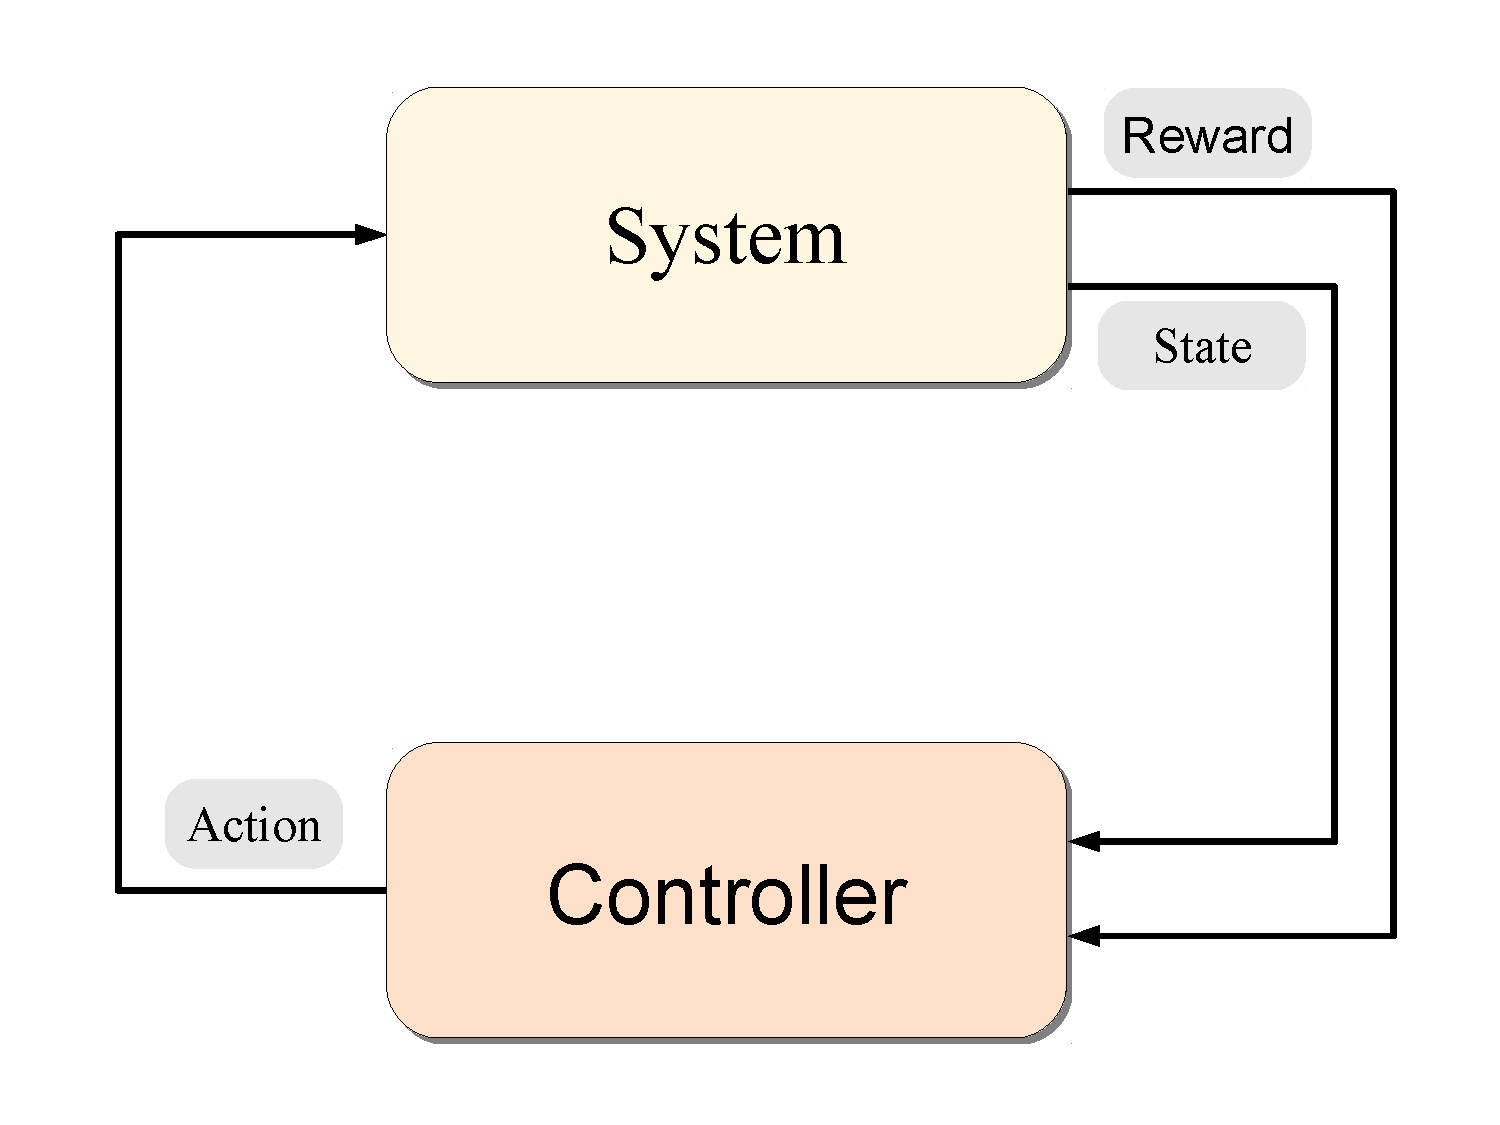
\includegraphics[width=0.5\textwidth]{Figures/ClosedLoopControl}
		%\hspace*{0.2in}
		%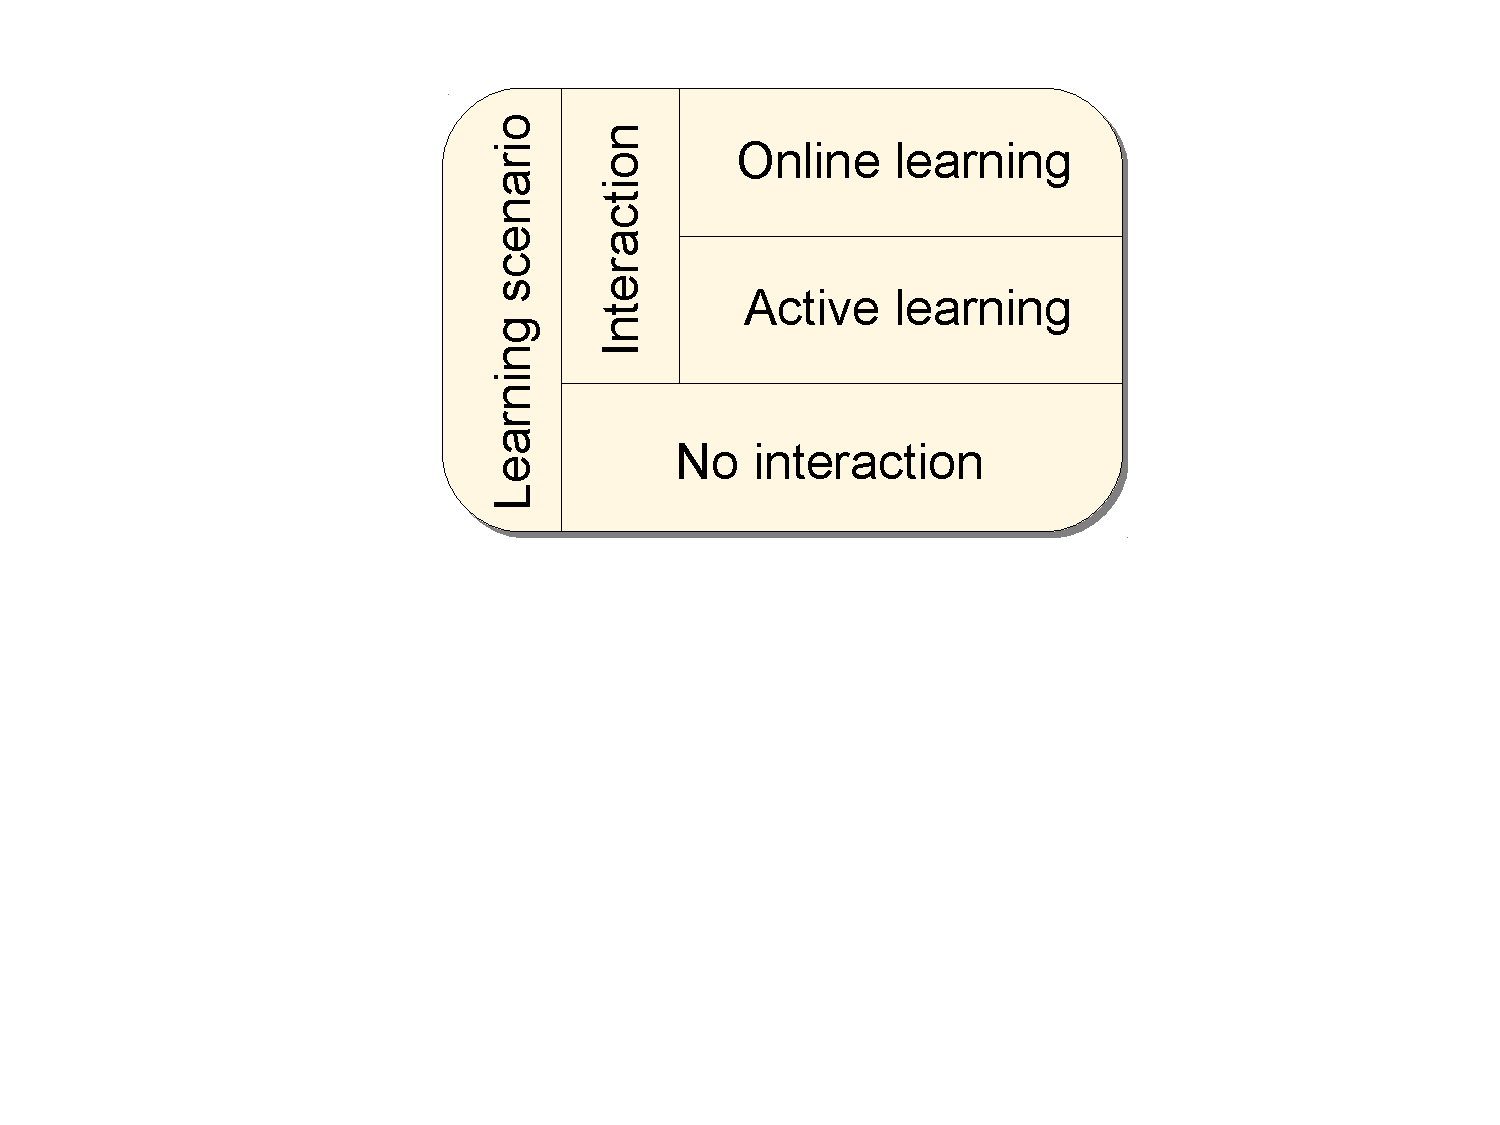
\includegraphics{learning-scenarios}
	\end{center}
	\end{figure}
	\note{
	\bin
	\item Sequential decision making under uncertainty
	\item Long-term objective
	\item Numerical performance measure
	\item Learning! (to overcome the ``curse of modeling'')
	\item Other terminologies in use:
	\bi
	\item Agent, environment
	\item Plant, Controller (feedback, closed-loop)
	\ei
	\item The state is sometimes not observable but that should not bother us now
	\ei
	}
}


\myframe{Preview of coming attractions}
{
	\begin{figure}[tb]
	\begin{center}
	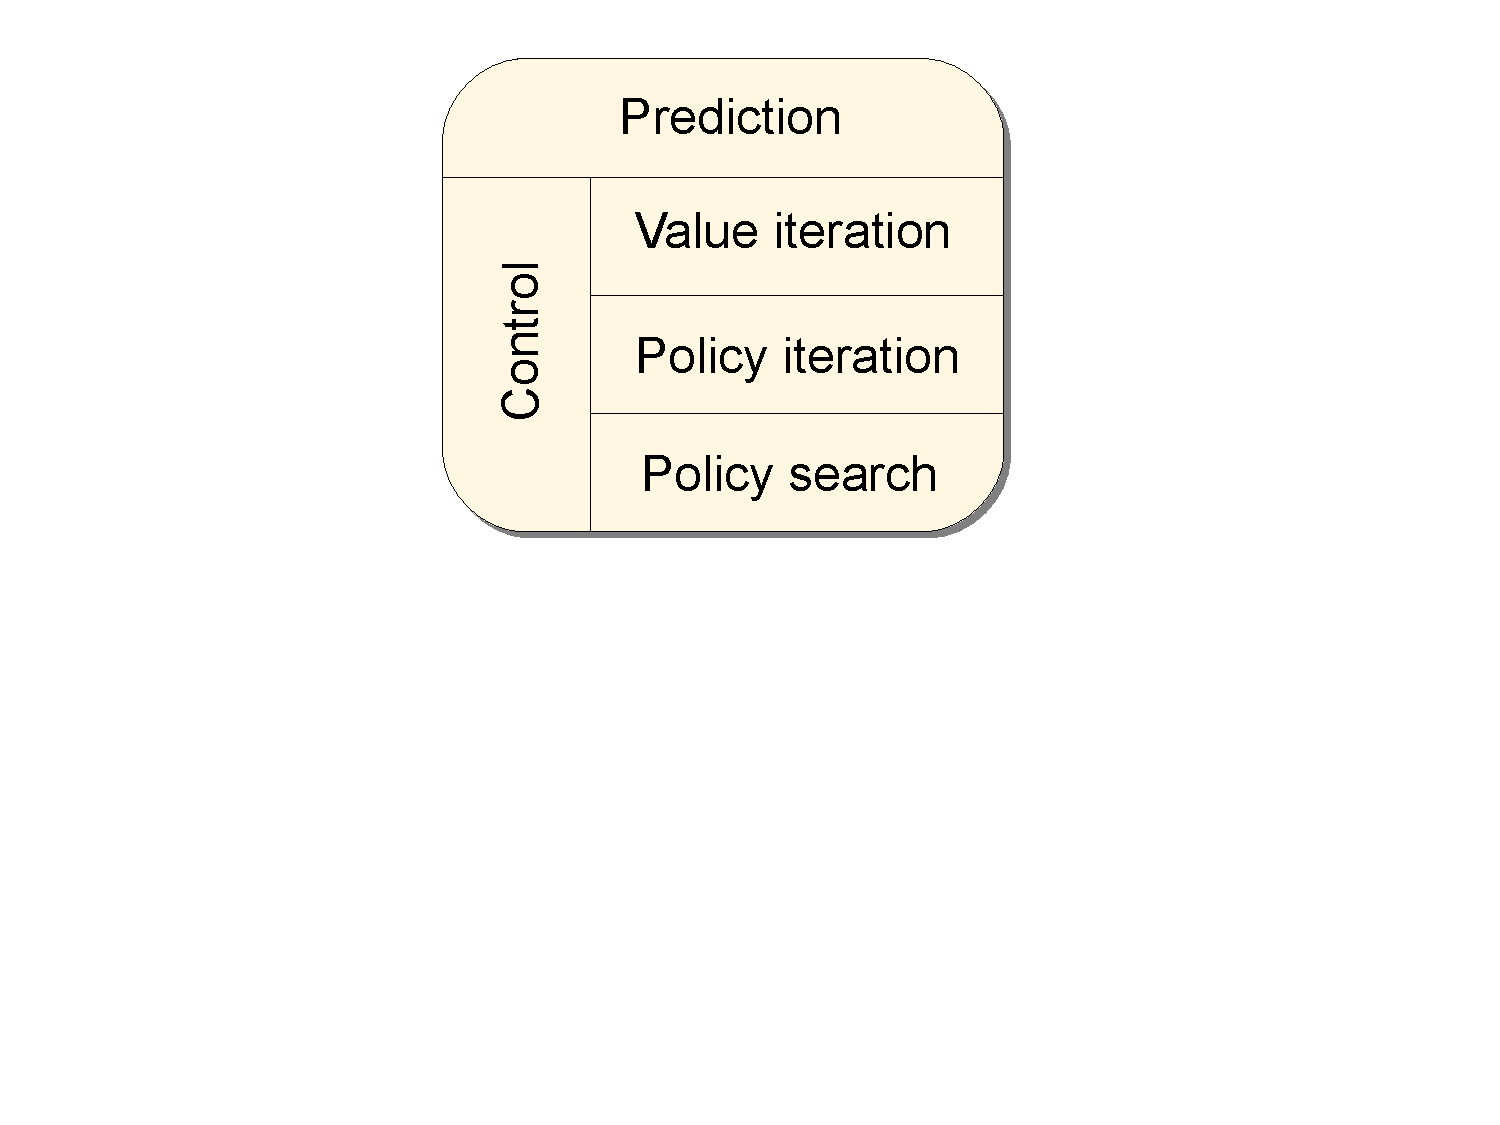
\includegraphics[width=0.5\textwidth]{Figures/problem-types}
		%\hspace*{0.2in}
		%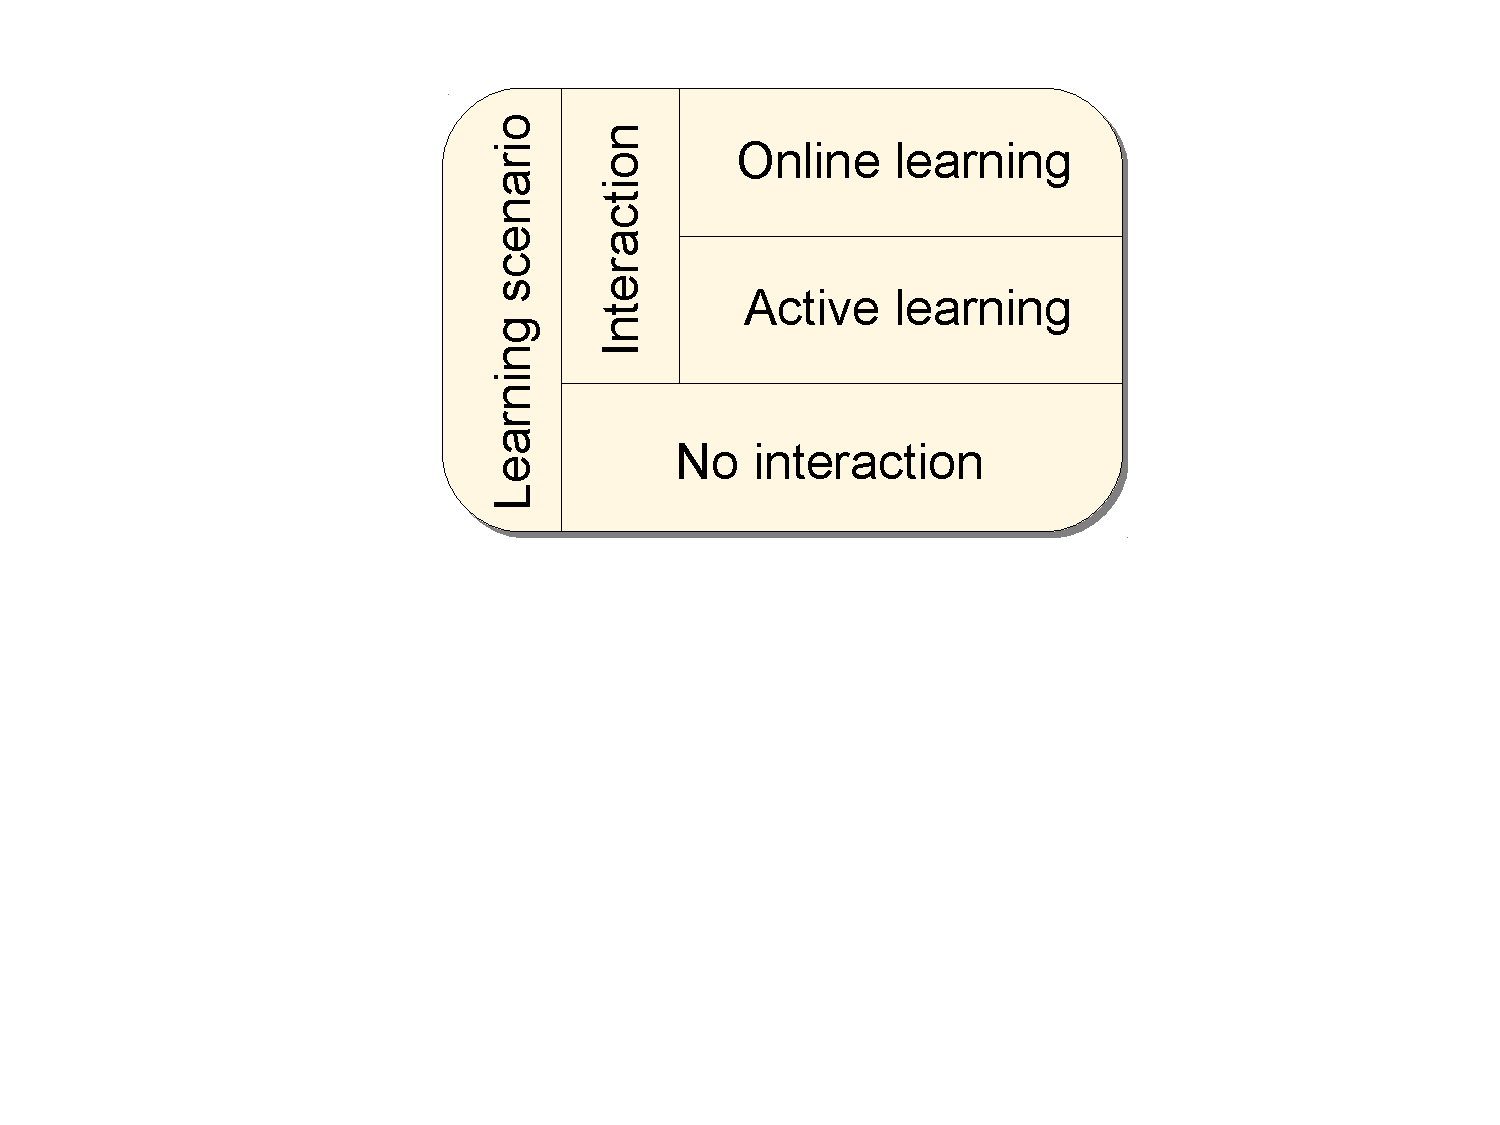
\includegraphics{learning-scenarios}
	\end{center}
	\end{figure}
	\note{
	\bin
	\item The structure of the talk follows this.
	\item Except that first we  introduce the framework of MDPs
	\ei
	}
}

\animframen{The structure of the tutorial}
{
\bi
\item Markov decision processes
\bi
\item Generalizes shortest path computations
\item Stochasticity, state, action, reward, value functions, policies
\item Bellman (optimality) equations, operators, fixed-points
\item Value iteration, policy iteration
\ei
\item Value prediction
\bi
\item Temporal difference learning unifies Monte-Carlo and bootstrapping
\item Function approximation to deal with large spaces
\item New gradient based methods %overcome previous limitations
\item Least-squares methods
\ei
\item Control
\bi
\item Closed-loop interactive learning: exploration vs. exploitation
\item $Q$-learning
\item SARSA
\item Policy gradient, natural actor-critic
\ei
\ei
\note{
Mention that we will see quite a few applications along the way.
}
}



\section{Markov decision processes}

\subsection{Motivating examples}
\myframe{How to get to Atlanta?}
{
	\begin{figure}[tb]
	\begin{center}
	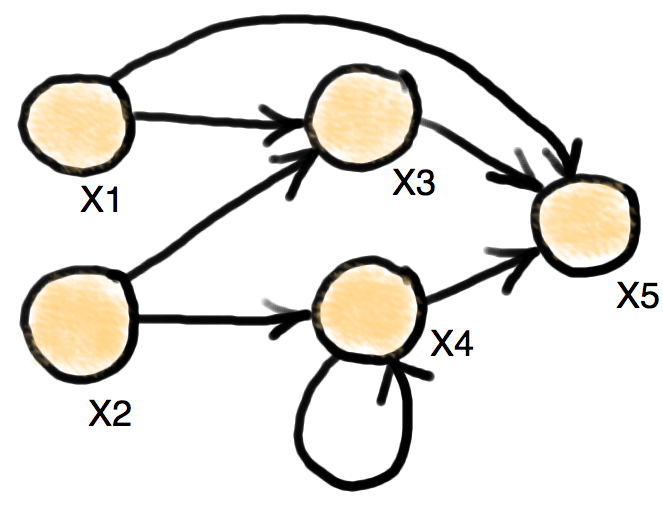
\includegraphics[width=0.5\textwidth]{Figures/graph00.png}
	\end{center}
	\end{figure}
	\note{
	\bin
	\item Story: How do you decide what is the shortest (fastest, cheapest, etc.) way to get to AAAI?
	\item[] (if you do not have a secretary)
	\item Consider the alternatives! 
	\item There are many many paths!!
	\item How to find the shortest one in an efficient manner?
	\item Let the audience think.. They should answer this question really..
	\item Then solve the shortest path problem by hand, by computing
	 the optimal \alert{cost-to-go} values, with full backups, following the ordering of nodes shown
	\item The goal is the node at the right that does not have any out edge.
	\ei
	}
}

\myframe{How to get to Atlanta?}
{
	\begin{figure}[tb]
	\begin{center}
	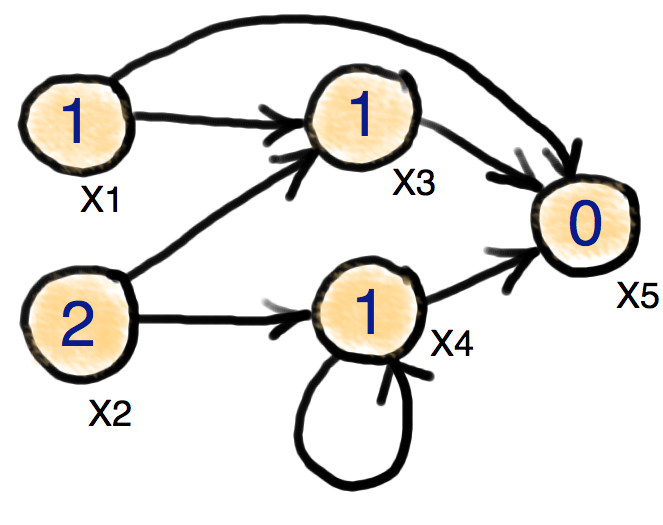
\includegraphics[width=0.5\textwidth]{Figures/graph01.png}
	\end{center}
	\end{figure}
	\note{
	\bin
  	 \item Mention that extension to non-uniform costs is trivial
	 \item Except when some of the costs could be negative
	 \item Assume that some costs can be negative. 
	 \item[] \alert{Homework}: when will the algorithm work?
	 \item[] Give examples when it does work and when it does not work!
	 \item \alert{Solution}: Two conditions:
	 \bi
	   \item There should be no ``free lunch''
	   \bi
	     \item ``Free lunch'' $\equiv$ $\exists$ 
	     policy that does not reach the goal state 
	     \item[] yet it has less than infinite cost from \alert{each} state
	   \ei
	   \item There should be at least one policy that reaches the goal
	 \ei
	\ei
	}
}

\begin{frame}[c]
\frametitle{Value iteration}

  \bcol[c]
  \col[0.4\textwidth]
	\begin{figure}[tb]
		\begin{center}
		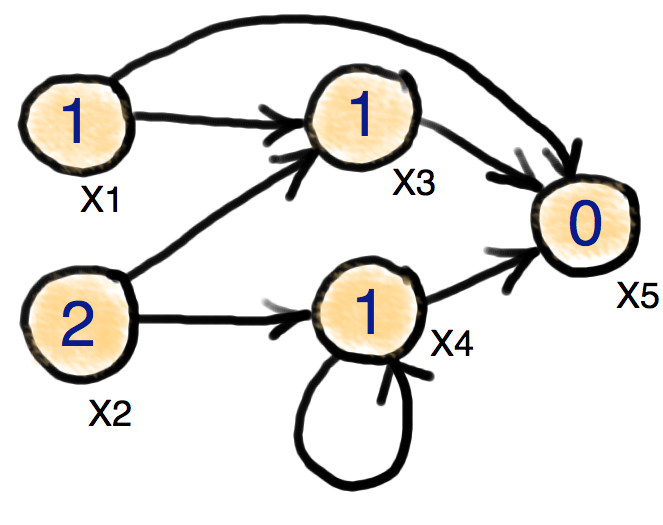
\includegraphics[width=0.8\textwidth]{Figures/graph01.png}
		\end{center}
	\end{figure}
  \col[0.6\textwidth]
        \begin{algorithmic}[1]
	        \Statex \mbox{} \hspace*{-2em} {\bf function} \Call{ValueIteration}{$\st^*$} 
		\State {\bf for} $\st\in\States$ {\bf do} $V[\st] \gets 0$
		\State $V' \gets V$
		\Repeat
			\For{$\st\in\States\setminus\{\st^*\}$}
				\State $V[\st] \gets 1 + \min_{\nextstate\in {\cal N}(\st)} V(\nextstate)$
			\EndFor
		\Until{$V\not= V'$}
		\State \Return $V$
	\end{algorithmic}
  \ecol

	\bigskip
	\bigskip
	
	\bcol
	\col[0.5\textwidth]
	\uncover<2->{
	   \begin{algorithmic}[1]
	        \Statex \mbox{} \hspace*{-2em} {\bf function} \Call{BestNextNode}{$\st,V$} 
	        \State \Return $\arg\min_{\nextstate\in {\cal N}(\st)} V(\nextstate)$
           \end{algorithmic}
	}
	\ecol
  \note{
  \bin
  \item Go through the algorithm
  \item Discuss how to decide which way to go to stay on the shortest path
  \item Introduce \alert{greedy choice}
  \item Introduce \alert{state}, \alert{action}
  \item Introduce \alert{policy}, i.e., stationary deterministic policy
  \ei
  }
\end{frame}


\begin{frame}
\frametitle{Rewarding excursions}

  \bcol[t]
  \col[0.7\textwidth]
        \begin{algorithmic}[1]
	        \Statex \mbox{} \hspace*{-2em} {\bf function} \Call{ValueIteration}{} 
		\State {\bf for} $\st\in\States$ {\bf do} $V[\st] \gets 0$
		\State $V' \gets V$
		\Repeat
			\For{$\st\in\States\setminus\{\st^*\}$}
				\State \hspace*{-0.1in} $V[\st] \gets  \displaystyle\max_{\action\in \Actions(\st)}\,\left\{\, \rewardfun(\st,\action) + \alert{\gamma}\,
					V(\, \alert{f}(\st,\action)) \,\right\}$
			\EndFor
		\Until{$V\not= V'$}
		\State \Return $V$
	\end{algorithmic}
	\col[0.3\textwidth]
	\begin{figure}[tb]
		\begin{center}
		\vspace*{-0.4in}
		\hspace*{-0.4in}
		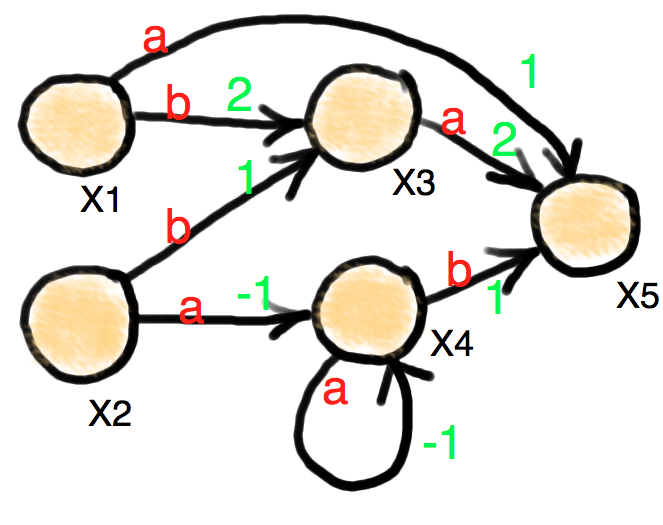
\includegraphics[width=1.2\textwidth]{Figures/graph02.png}
		\end{center}
	\end{figure}	
  \ecol

	\bigskip
	\bigskip
	
	\bcol
	\col[0.7\textwidth]
	\uncover<2->{
	   \begin{algorithmic}[1]
	        \Statex \mbox{} \hspace*{-2em} {\bf function} \Call{BestAction}{$\st,V$} 
	        \State \Return $ \displaystyle\argmax_{\action\in \Actions(\st)}\,\left\{\, \rewardfun(\st,\action) + \alert{\gamma}\,
					V(\, \alert{f}(\st,\action)) \,\right\}$
           \end{algorithmic}
	}
	\col[0.3\textwidth]
	\ecol

	\note{
	\bin
	\item Introduce \alert{rewards}
	\item Introduce \alert{transition function} $f$
	\item Introduce \alert{discounting}: 
	\bi
	\item One dollar in the future worth less than today. 
	\item In general, the future is important but maybe not as important as today
	\item Write $\sum_{t=0}^\infty \gamma^t R_t$
	\item Economics: $\gamma = 1/(1+\rho)$, where $0<\rho\ll 1$ is the interest rate. 
	\ei
	\ei
	}
\end{frame}

\myframen{Uncertainty}
{
\bcol[t]
\col[0.8\textwidth]
\begin{quote}
``Uncertainty is the only certainty there is, and knowing how to live with insecurity is the only security.'' (John Allen Paulos, 1945--)
\end{quote}
\col[0.2\textwidth]
\bc
\vspace*{-1in}

\includegraphics[width=1in]{Figures/smjap.jpg}
\ec
\ecol
\vspace*{-0.5in}
	\bi[<+->]
	\item Next state might be uncertain
	\item The reward detto
	\item Advantage: Richer model, robustness
	\item A transition from $\St$ after taking action $\Action$:
	\beqan
	\Nextstate &=& f(\St,\Action,D),\\
	\Reward    &=& g(\St,\Action,D)
	\eeqan
	\item $D$ -- random variable; ``\alert{disturbance}''
	\item $f$ -- \alert{transition function}
	\item $g$ -- \alert{reward function}
	\ei
	
	\note{
	\bin
	\item John Allen Paulos, \url{http://www.math.temple.edu/~paulos/}, 
	John Allen Paulos is an extensively  ``kudized'' author, popular public speaker, and monthly columnist for ABCNews.com and formerly for the Guardian. Professor of math at Temple. Funny guy, has interesting thoughts:)
	\item In the previous graph we could have actions, instead of edges and then stochastic transitions out from the nodes.
	\ei
	}
}



{
\usebackgroundtemplate{
\includegraphics[width=\paperwidth]{Figures/worldlightmap.jpg}}
\animframen{Power management}
{
%\putat{300}{50}{
\includegraphics[width=0.5in]{Figures/100px-Energy_Star_logo.png}}
\note{
\bin
\item Blurb about how important is power management
\ei
\begin{quotation}
The monumental number of PCs operating worldwide creates other requirements for PC power management. Because there are hundreds of millions of PCs in operation, the installed base of computers worldwide consumes \alert{tens of gigawatts for every hour} of operation. Even small changes in average desktop computer power consumption can, on the global scale, save as much power as generated by a small power plant. ({\em Source: Intel}, \url{http://www.intel.com/intelpress/samples/PPM_chapter.pdf})
\end{quotation}
}
}
}

\animframen{Computer usage data}
{

\includegraphics[width = 0.5\textwidth]{Figures/AMD-data-home}

\includegraphics[width = 0.5\textwidth]{Figures/AMD-data-office}

% 128mm x 96mm
\putatUL{\textwidth}{0mm}{80mm}
{
\begin{center}
\tiny
Source:
\url{http://www.amd.com/us/Documents/43029A_Brochure_PFD.pdf}
\end{center}
}


\note{
\bin
\item
Background:
AMD surveyed over 1200 users to determine consumer and commercial usage patterns (daily time spent on each application or at idle) in four countries.
\item What is important:
\bi
\item Computers are often idle 
\item They do all kind of works at other times, which require different parts of the computer to be awake
\item Why is power management challenging?
\bi
\item Everyone uses the computer differently.
\item One size fits all?? NO!
\ei
\ei
\ei
}
}

\begin{frame}
\frametitle{Power management}
\putat{300}{50}{
\includegraphics[width=0.5in]{Figures/100px-Energy_Star_logo.png}}
\bi
\item {\bf Advanced Configuration and Power Interface (ACPI) }
\item First released in December 1996, last release in June 2010
\item Platform-independent interfaces for hardware discovery, configuration, power management and monitoring
\ei
\note{
This is a complex issue. This will be illustrated on the next two slides. 
The details on these slides are not so important. However, they illustrate well the complexity of the issue.
}
\end{frame}


\animframesqn{Power mgmt -- Power states}
{
\bi
  \item G0 (S0): Working
  \item G1, Sleeping subdivides into the four states S1 through S4 
     \bi
	\item S1: All processor caches are flushed, and the CPU(s) stop executing instructions. 
	Power to the CPU(s) and RAM is maintained; devices that do not indicate
	 they must remain on may be powered down
	\item S2: CPU powered off
	\item S3: Commonly referred to as Standby, Sleep, or Suspend to RAM. RAM  remains powered
	\item S4: Hibernation or Suspend to Disk. 
	All content of main memory is saved to non-volatile memory such as a hard drive, and is powered down
     \ei
  \item G2 (S5), Soft Off: G2 is almost the same as G3 Mechanical Off, 
  but some components remain powered so the computer can 
  "wake" from input from the keyboard, clock, modem, LAN, or USB device.
  \item G3, Mechanical Off: The computer's power consumption approaches close to zero, 
  to the point that the power cord can be removed and the system is safe for dis-assembly 
  (typically, only the real-time clock is running off its own small battery).
\ei
}
\myframesqn{Power mgmt -- Device, processor, performance states}
{
\bi
\item Device states
	\bi
	\item D0 Fully-On is the operating state
	\item D1 and D2 are intermediate power-states whose definition varies by device.
	\item D3 Off has the device powered off and unresponsive to its bus.
	\ei
\item Processor states
	\bi
	\item C0 is the operating state.
	\item C1 (often known as Halt) is a state where the processor is not executing instructions, but can return to an executing state essentially instantaneously. All ACPI-conformant processors must support this power state. Some processors, such as the Pentium 4, also support an Enhanced C1 state (C1E or Enhanced Halt State) for lower power consumption.
	\item C2 (often known as Stop-Clock) is a state where the processor maintains all software-visible state, but may take longer to wake up. This processor state is optional.
	\item C3 (often known as Sleep) is a state where the processor does not need to keep its cache coherent, but maintains other state. Some processors have variations on the C3 state (Deep Sleep, Deeper Sleep, etc.) that differ in how long it takes to wake the processor. This processor state is optional.
	\ei
\item Performance states: While a device or processor operates (D0 and C0, respectively), it can be in one of several power-performance states. These states are implementation-dependent, but P0 is always the highest-performance state, with P1 to Pn being successively lower-performance states, up to an implementation-specific limit of n  no greater than 16.
\item[] P-states have become known as SpeedStep  in Intel processors, as PowerNow! or Cool'n'Quiet in AMD processors, and as PowerSaver in VIA processors.
\bi
\item P0 max power and frequency
\item P1 less than P0, voltage/frequency scaled
\item Pn less than P(n-1), voltage/frequency scaled
\ei
\ei
}

\animframen{An oversimplified model}
{
\begin{figure}
\begin{center}
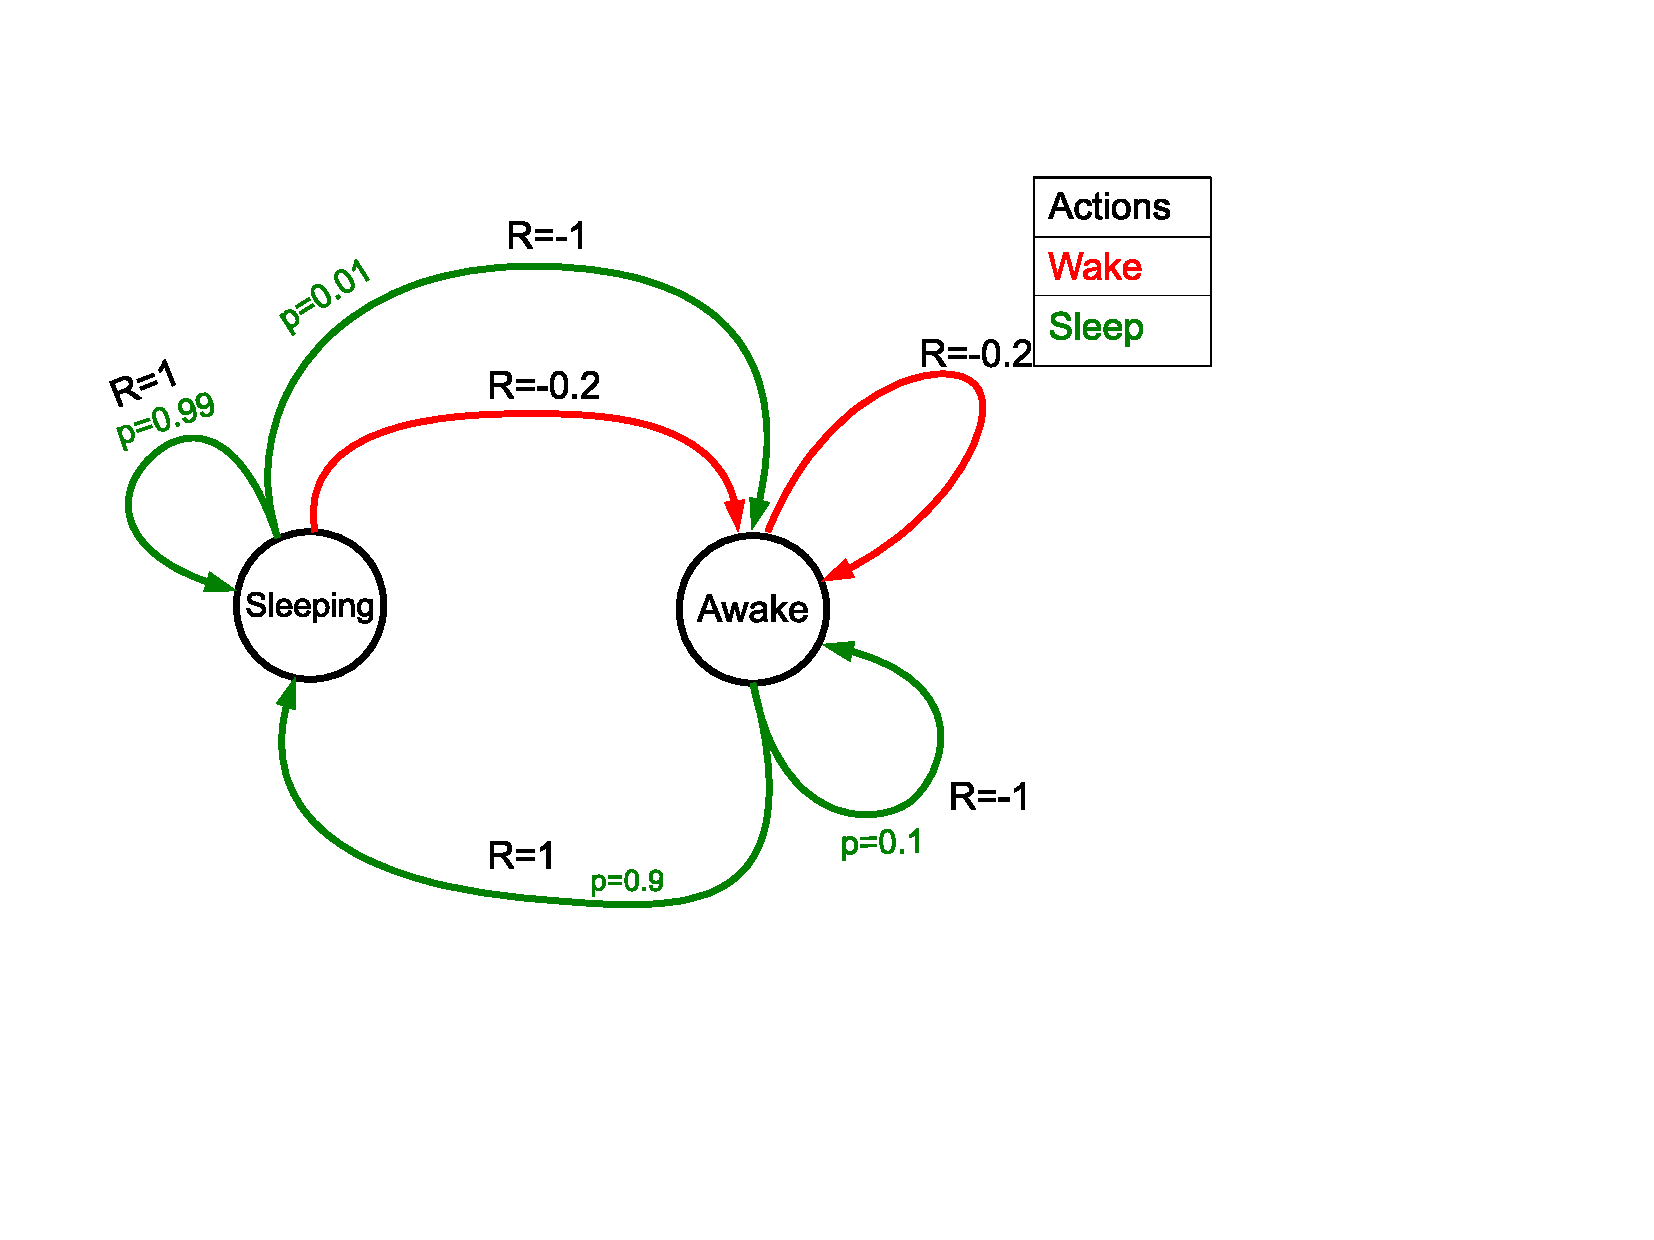
\includegraphics[width=0.5\textwidth]{Figures/Sleep-Wake}
\end{center}
\end{figure}
\begin{Note}<2->
The transitions can be represented as 
\beqan
\Nextstate &=& f(\st,\action,D),\\
\Reward    &=& g(\st,\action,D).
\eeqan
\end{Note}
\note{
 \bin
 \item This is indeed oversimplified
 \item We could have more states
 \item $\ldots$ but the message should be clear.
 \ei
}
}

\begin{frame}
\frametitle{Value iteration}
	\putat{200}{-70}{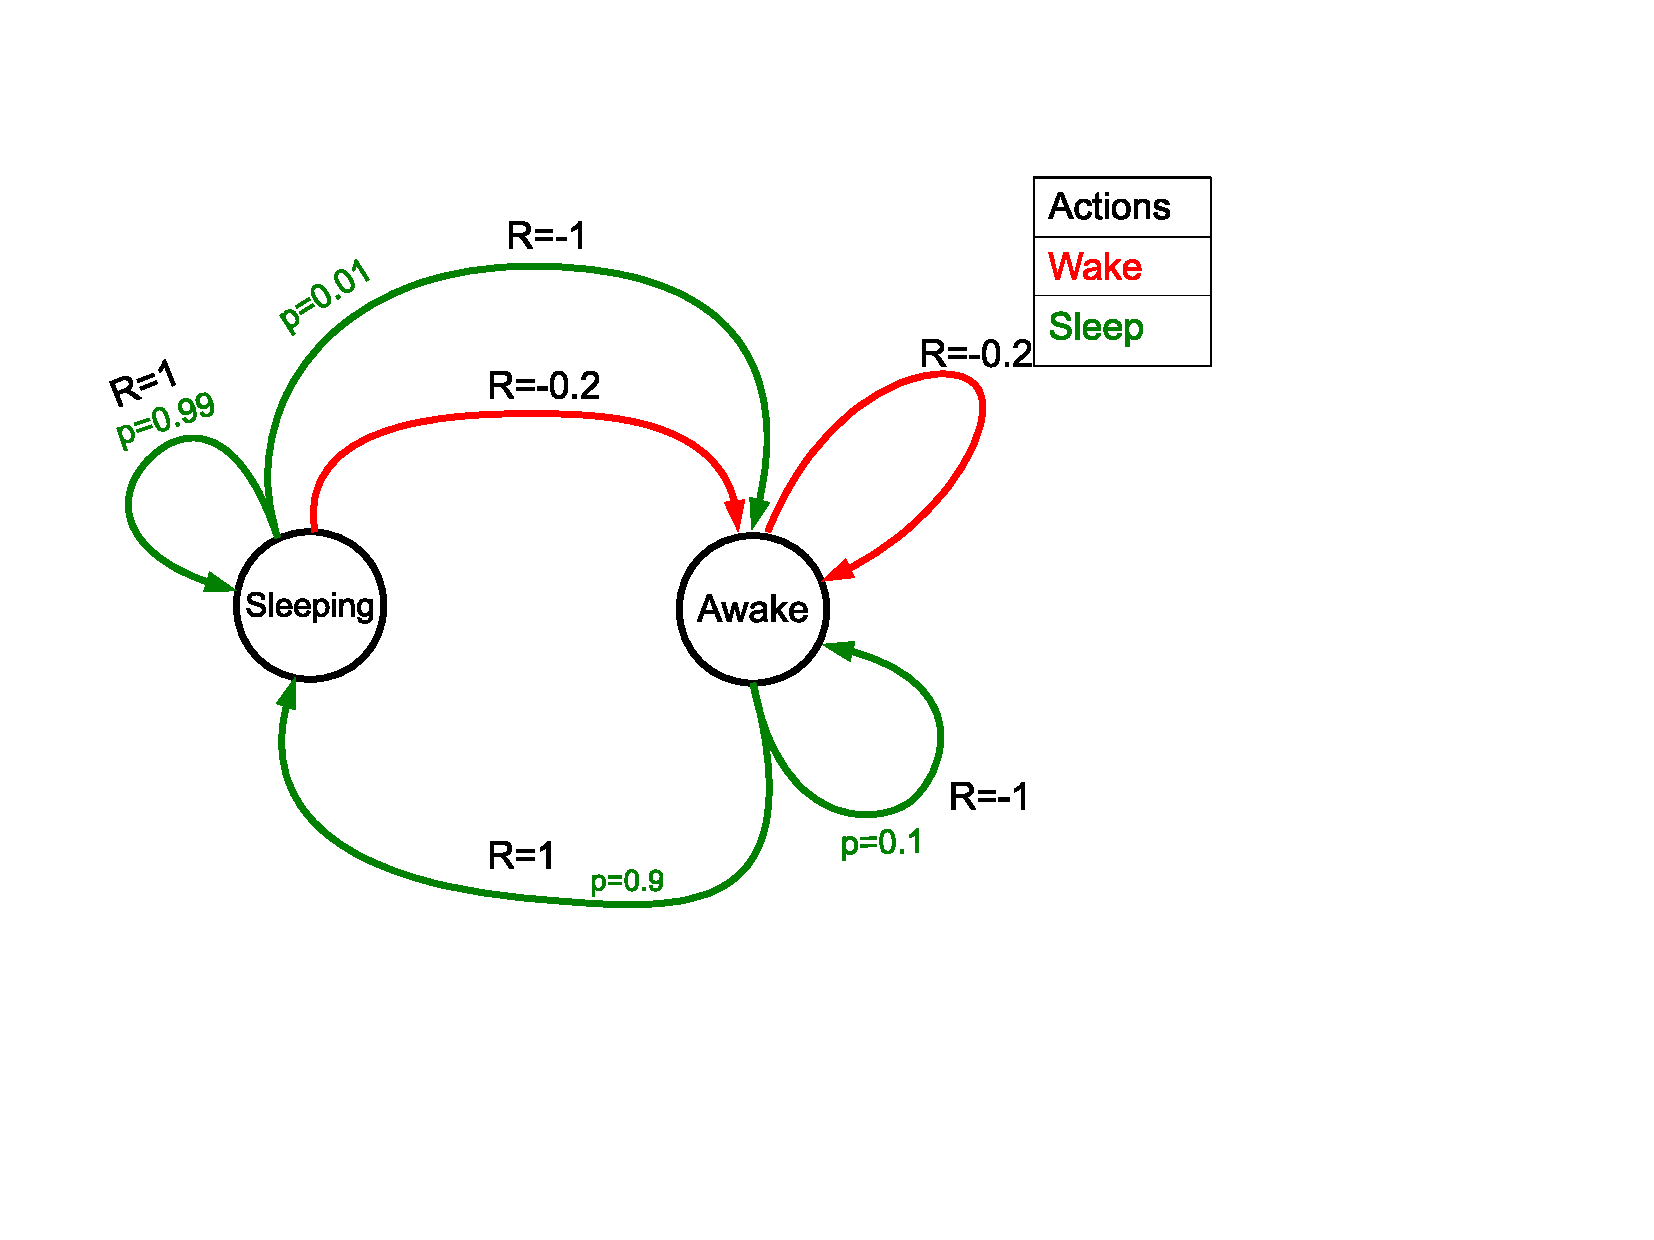
\includegraphics[width=2in]{Figures/Sleep-Wake}}

  \bcol[t]
  \col[0.8\textwidth]
        \begin{algorithmic}[1]
	        \Statex \mbox{} \hspace*{-2em} {\bf function} \Call{ValueIteration}{} 
		\State {\bf for} $\st\in\States$ {\bf do} $V[\st] \gets 0$
		\State $V' \gets V$
		\Repeat
			\For{$\st\in\States\setminus\{\st^*\}$}
				\State \hspace*{-0.1in} $V[\st] \gets 
				 \displaystyle\max_{\action\in \Actions(\st)}\,
				\EE{ \alert{g}(\st,\action,\alert{D}) + \gamma \,
					V(\, \alert{f}(\st,\action,\alert{D}))  \,}$
			\EndFor
		\Until{$V\not= V'$}
		\State \Return $V$
	\end{algorithmic}
	\col[0.2\textwidth]
  \ecol

	\bigskip
	\bigskip
	
	\bcol
	\col[0.7\textwidth]
	\uncover<2->{
	   \begin{algorithmic}[1]
	        \Statex \mbox{} \hspace*{-2em} {\bf function} \Call{BestAction}{$\st,V$} 
	        \State \Return $ 
	         \displaystyle\argmax_{\action\in \Actions(\st)}\,
				\EE{ \alert{g}(\st,\action,\alert{D}) + \gamma \,
					V(\, \alert{f}(\st,\action,\alert{D}))  \,}$
           \end{algorithmic}
	}
	\col[0.3\textwidth]
	\ecol

	\note{
	\bin
	\item Straightforward generalization of previous algorithm: 
	\item[] In each step we compute the expected total reward based on the assumption that the total
	future rewards are given by $V$
	\item \alert{Homework}: Think about the stochastic shortest path case and convince yourself that this works.
	\item Question: Why does it work in general? \alert{POSTPONED!}
	\item Show how the computation is done $\Leftarrow$ Excel sheet!
	\item \alert{IMPORTANT}: 
		Uncertainty makes it necessary to check back where you are! In deterministic problems, knowing the initial state is enough to know how to act until you get to your goal!
	\ei
	}
\end{frame}






\animframen{How to gamble if you must?}
{
	\begin{quote}
	The safest way to double your money is to fold it over once and put it in your pocket.  (``Kin'' Hubbard, 1868--1930)
	\end{quote}

\bi
\item State $\St_t$ $\equiv $ wealth of gambler at step $t$,  $\St_t\ge 0$
\item Action: $\Action_t\in [0,1]$: the fraction of $\St_t$ put at stake
\item $S_t\in \{-1,+1\}$, $\Prob{S_{t+1}=1} = p$, $p\in [0,1]$, i.i.d., random variables
\item Fortune at next time step:
\[
\St_{t+1} = 
(1+S_{t+1}\Action_t) \St_t.
\]
\item \alert{Goal}:  maximize the probability that the wealth reaches $w^*$.
\item How to put this into our framework?
\ei

	
\note{
\bin
\item 
Frank McKinney Hubbard is
an American cartoonist, humorist, and journalist  better known by his pen name "Kin" Hubbard.
\item Imagine e.g. that as a last resort you have to bet on horses because you just need to money to pay back your debt to the mafia or you die.
\ei
}

}
\animframen{How to gamble if you must? -- Solution}
{
\bi
\item $\St_t \in \States = [0,w^*]$, $\Actions = [0,1]$
\item Let $f:\States \times \Actions\times \{-1,+1\} \ra \States$ be
\[
f(\st,\action,s) = \begin{cases}
(1+ s \, \action) \st \wedge w^*, & \text{ if } \st<w^*;\\
w^*, & \text{ otherwise}.
\end{cases}
\]
\item Let $g:\States \times \Actions\times \{-1,+1\} \ra \States$ be
\[
g(\st,\action,s) = \begin{cases}
1, & \text{ if } (1+ s\, \action) \st\ge w^* \text{ and } \st<w^*;\\
0, & \text{ otherwise}.
\end{cases}
\]
\item What is the optimal policy?
\ei
\note{
\bin
\item Mention that this is an \alert{episodic problem}
\item The strange tent-like symbol, $\wedge$, is a binary operator, similar to, say, $+$. It computes the minimum of its arguments.
\item Here $w^*$ is an \alert{absorbing state}
\item This is a prototypical example of how we can deal with problems when the goal is to maximize the probability of an event
\item Ask audience: How would you play this game?
\item How to compute the optimal value function?
\item[] The state space became infinite..
\item Optimal strategy: ``bold strategy'' (no need to tell them)
\bi
\item Risk the smallest of the amount missing to reach $w^*$ and your current wealth
\ei
\ei
}
}


\animframen{Inventory control}
{
\begin{figure}
\begin{center}
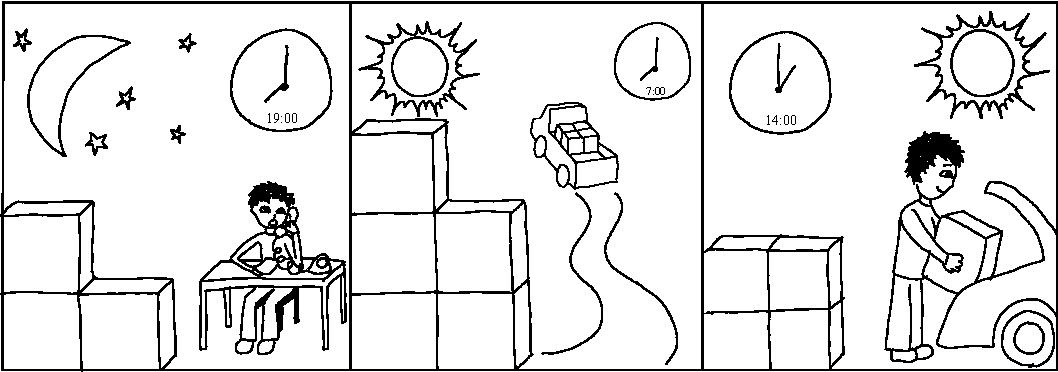
\includegraphics[width=0.8\textwidth]{Figures/inventory-mgmt}
\end{center}
\end{figure}

\bc
\scaletext{0.7}{1.1}{
	\bi[<+->]
	\item $\States = \{0,1,\ldots,M\}$; $\St_t$ size of the inventory in the evening of day $t$
	\item $\Actions = \{0,1,\ldots,M\}$; $\Action_t$ number of items ordered in the evening of day $t$
	\ei
	\uncover<+->{
	Dynamics:
	\[
	\St_{t+1} = ((\St_t + A_t ) \wedge M - D_{t+1} )^+.
	\]}
	\uncover<+->{
	Reward:
	\[
	\begin{split}
	\Reward_{t+1} &= 
	 -  K \,\one{A_t>0}  
	- c \, ( (\St_t + A_t ) \wedge M - \St_t )^+\\
	&\quad 
	 - h\, \St_t
	\qquad 
	+ p \,( (\St_t + A_t ) \wedge M- \St_{t+1})^+.
	\end{split}
	\]
	}
}
\ec

\note{
\bin
\item Explanation of the quantities involved:
\bi
\item $M$ -- maximum inventory size
\item $D_{t+1}$ -- demand
\item $K$ -- fixed cost of ordering any items
\item $c$ -- cost of lost sales
\item $h$ -- inventory cost
\item $p$ -- sales proceeds
\ei
\item  $Z_t = (X_t+A_t) \wedge M$ -- \alert{post-decision state}, or \alert{afterstate}
\item[] This also comes up in \alert{games}
\ei
}
}

\myframen{Other examples}
{
\bi
\item Engineering, operations research
\bi 
\item Process control
\bi
\item Chemical
\item Electronic
\item Mechanical systems $\Ra$ ROBOTS
\ei
\item Supply chain management
\ei
\item Information theory 
\bi
\item optimal coding
\item channel allocation
\item sensing, sensor networks
\ei
\item Finance
\bi
\item portfolio management
\item option pricing
\ei
\item Artificial intelligence
\bi
\item The whole problem of acting under uncertainty
\item Search
\item Games
\item Vision: Gaze control
\item Information retrieval
\ei
\item $\vdots$
\ei
\note{
\bin
\item The point is, these problems are ubiquous.
\item TODO: Add some figures
\ei
}
}

\subsection{Controlled Markov processes}

\animframen{Controlled Markov processes}
{
	\vspace*{-0.2in}
	\begin{align*}
	\begin{split}
		\St_{t+1} &= f(\St_t,\Action_t,D_{t+1}) \qquad \uncover<+->{\text{State dynamics}}\\
		\vspace*{0.1in}
		\uncover<+->{
		\Reward_{t+1} &= g(\St_t,\Action_t,D_{t+1})} \qquad \uncover<+->{\text{Reward}}\\
		\vspace*{0.1in}
		 &\quad \uncover<+->{t=0,1,\ldots\,.}
	\end{split}
	\end{align*}
	
	\bigskip

\hspace*{0.8in}{
\begin{minipage}[h]{\textwidth} 
	\bi[<+->]
	\item $\St_t\in \States$ -- state at time $t$
	\item $\States$ -- set of states
	\item $\Action_t\in \Actions$ -- action at time $t$
	\item $\Actions$ -- set of actions 
	\item Sometimes, $\Actions(\st)$: \alert{admissible actions}
	\item $\Reward_{t+1}\in \real$ -- reward $\Ra$ $\Real$
	\item $D_t\in {\cal D}$ -- disturbance; \alert{i.i.d.} sequence
	\item ${\cal D}$ -- disturbance space
	\ei
%	}
%	\ecol
\end{minipage}
}

\note{This just collects on a single slide what we have talked about before.}
}

\animframen{Return}
{
\begin{Definition}[Return]
Return, or total discounted return is:
\[
\Ret = \sum_{t=0}^\infty \gamma^t \Reward_{t+1},
\]
where $0\le \gamma \le 1$ is the so-called \alert{discount factor}.
The return depends on how we act!
\end{Definition}

\note{
\bin
\item The return is an important quantity.
\item Return $\not=$ immediate reward (or, just reward)
\item The index goes fro time step zero, but the ``zero'' can be shifted around
\item If the rewards are bounded in expectation and the discount factor $\gamma$ is less than one then the expected return is well defined.
\item If the rewards can be unbounded (from below, or above), care must be taken, e.g., Gaussian noise..
\item The discount factor could be one, but then one must be careful because the return might become unbounded, even when the rewards are bounded
\ei
}
}

\animframen{The goal of control}
{
	\begin{block}{Goal}
	Maximize the \alert{expected total discounted reward}, 
	or \alert{expected return}, irrespective of the initial state:
	\[
	\EE{ \sum_{t=0}^\infty \gamma^t \Reward_{t+1} \,|\, \St_0 = \st} \ra \max!, \quad \st\in\States. 
	\]
	\end{block}

\note{
\bin
\item Note that there is no distribution over the states.
\item We want to act optimally from \alert{each} state
\item For each state, a different ``policy'' might be optimal.
\ei
}
}


\subsection{Alternate definitions}
\animframen{Alternate definition}
{
\begin{Definition}[Markov decision process]
Triplet: $(\States,\Actions,\JTranKernel)$, where 
\bi[<+->]
\item $\States$ -- set of states
\item $\Actions$ -- set of actions
\item $\JTranKernel$ -- state and reward kernel
\item[] $\JTranKernel(U|\st,\action)$ is the probability that $(\St_{t+1},\Reward_{t+1})$ lands in $U\subset \States\times \real$ given that $\St_t = \st$, $\Action_t = \action$
\ei
\end{Definition}

\note{
\bin
\item Somewhat unconventional definition, but very compact at least, \\and very general, too
\ei
}
}

\animframen{Connection to previous definition}
{
Assume that
	\begin{align*}
	\begin{split}
		\St_{t+1} &= f(\St_t,\Action_t,D_{t+1}) \\
		\Reward_{t+1} &= g(\St_t,\Action_t,D_{t+1})\\
		 &\quad t=0,1,\ldots\,.
	\end{split}
	\end{align*}

Then
\[
\JTranKernel(U|\,\st,\action) = \Prob{ \,\,[\,f(\st,\action,D),g(\st,\action,D)] \in U\,\, },
\]

Here, $D$ has the same distribution as $D_1,D_2,\ldots$.

\note{
\bin
\item
The two definitions, in fact, are equivalent.
\item
Sometimes this, sometimes the other definition is the more convenient
\ei
}
}

\animframen{``Classical form''}
{
Finite MDP (as is often seen in AI publications):
\[
(\States,\Actions,\TranKernel,\rewardfun)
\]

\bi[<+->]
\item $\States,\Actions$ are finite.
\item $\TranKernel( \st,\action, \nextstate )$ is the probability of landing at state $\nextstate$ 
given that action $\action$ was chosen in state $\st$
\item $\rewardfun(\st,\action,\nextstate)$ is the expected reward received 
when making this transition.
\ei

\note{
\bin
\item This is a smaller class
\item But if $\States$, $\Actions$ are allowed to be countably infinite, the analysis can get pretty complicated.
\item What is lost is our ability to talk about continuity:
\bi
\item The naming of states, actions is arbitrary!!
\item In continuous problems, we often have some sort of continuity, allowing for generalization to ``nearby'' states/actions!
\item This could be mimicked by introducing some kind of ``distance function''
\ei
\ei
}
}

\subsection{Policies, values}
\animframen{Policies, values}
{
\begin{Note}
From now on we assume that $\Actions$ is countable.
\end{Note}

\begin{Definition}[General policy]
Maps each history to a distribution over $\Actions$.

\noindent Deterministic policy:
$\pi = (\pi_0,\pi_1,\ldots)$, where
 $\pi_0:\States \ra \Actions$
 and $\pi_t : (\States \times \Actions\times \real)^{t-1} \times \States \ra \Actions$, $t=1,2,\ldots$.
 
 \noindent Following the policy:
 $\Action_t = \pi_t(\St_0,\Action_0,\Reward_1,\ldots,\St_{t-1},\Action_{t-1},\Reward_t,\St_t)$.
\end{Definition}

\note{
\bin
\item General policies: When we do learning, we follow a general policy, because the policy depends on the history!
\item Usually the history is compressed in some form
\ei
}

}
\animframen{Stationary policies}
{
\begin{Definition}[Stationary policy]
The map depends on the last state only.
\bi
\item
\alert{Deterministic policy}:
$\pi = (\pi_0,\pi_0,\ldots)$.
\item[]
 Following the policy:
 $\Action_t = \pi_0(\St_t)$.
\item
\alert{Stochastic policy}:
$\pi = (\pi_0,\pi_0,\ldots)$, $\pi_0: \States \ra M_1(\Actions)$.
\item[] Following the policy:
$\Action_t \sim \pi_0(\cdot|\St_t)$.
\ei
\end{Definition}


\note{
\bin
\item We just identify $\pi$ and $\pi_0$.
\item Stationary policies has a distinctive role in the theory of MDPs
\ei
}
}

\animframen{The value of a policy}
{
\begin{Definition}[Value of a state under $\pi$]
The expected return given that the policy is started in state $\st$:
\[
V^\pi(\st) = \EE{ \Ret^\pi | \St_0 = \st }.
\]
$V^\pi$ -- value function of $\pi$.
\end{Definition}
\begin{Definition}[Action-value of a state-action pair under $\pi$]
The expected return given that the process is started from state $\st$, the first action is $\action$ after which the policy $\pi$ is followed:
\[
Q^\pi(\st,\action) = \EE{ \Ret^\pi | \St_0 = \st,\Action_0 = \action }.
\]
$Q^\pi$ -- action-value function of $\pi$
\end{Definition}

\note{
\bin
\item These are well-defined under our conditions.
\item Even for general policies.
\item The action-values were introduced by Watkins; they are very useful as we shall see later.
\ei
}
}


\animframen{Optimal values}
{
\begin{Definition}[Optimal values]
The \alert{optimal value} of a state is the value of the best possible expected return that can be obtained from that state:
\[
V^*(\st) = \sup_{\pi} V^\pi(\st).
\] 
Similarly, the \alert{ optimal value } of a state-action pair is $Q^*(\st,\action) = \sup_{\pi} Q^\pi(\st,\action)$.
\end{Definition}
\begin{Definition}[Optimal policy]
A policy $\pi$ is called {\em optimal} if $V^\pi(\st) = V^*(\st)$ holds for all states $\st\in\States$.
\end{Definition}

\note{
\bin
\item The questions are:
\bin
\item Does there exist and optimal policy?
\item A simple optimal policy?
\item A computable optimal policy?
\item How to compute it?
\ei
\ei
}
}

\section{Theory of dynamic programming}
\subsection{The fundamental theorem}
\animframejsqn{The fundamental theorem { \small and the Bellman (optimality) operator}}
{
\small
\vspace*{-0.1in}
\begin{Theorem}
Assume that $|\Actions|<+\infty$.
Then the optimal value function satisfies
\[
V^*(\st) = \max_{\action\in\Actions} \left\{ \reward(\st,\action) + \gamma 
\sum_{\nextstate\in \States} \PKernel(\st,\action,\nextstate) V^*(\nextstate) \right\}, \quad\quad \st\in\States.
\]
and if policy $\pi$ is such that in each state $\st$ it selects an action  that maximizes the r.h.s. then $\pi$ is an optimal policy.
\end{Theorem}
\begin{block}{}
\small
\pgfputat{\pgfxy(10.3,0)}{\pgfbox[left,top]{
	\includegraphics[width=0.5in]<2->{Figures/Bellman.png}}
	}
A shorter way to write this is
\[
V^* = T^* V^*,
\]
%\putat{300}{-10}{
\includegraphics[width=0.5in]{Figures/Bellman.png}} % \\R.E.Bellman (1920--1984)}
%where $T^*$ is the so-called \alert{Bellman-operator}:
%\newcommand{\putat}[3]{\begin{picture}(0,0)(0,0)\put(#1,#2){#3}\end{picture}} % xrelpos yrelpos WHAT
\[
(T^* V)(\st) =\max_{\action\in\Actions} \left\{ \reward(\st,\action) + \gamma 
\sum_{\nextstate\in \States} \PKernel(\st,\action,\nextstate) V(\nextstate) \right\}, \quad \st\in\States.
\]
\end{block}
%\putat{300}{50}{
\includegraphics[width=0.5in]{Figures/100px-Energy_Star_logo.png}}
\note{
\bin
\item Explain that operators are just functions that act on functions, but functions are really like vectors, so no one should be afraid of this.
\item What is the history? Hard to tell. The theorem exists in various generalities. This simple form must have been known to Bellman (1920--1984), who ``invented'' dynamic programming in 1953.
Dreyfus, Blackwell and others worked out the math for the more complicated cases and there is still work left. Some older economics literature mentioned the principle of optimality.
\ei
}
}

\animframen{Action evaluation operator}
{
\begin{definition}[Action evaluation operator]
Let $\action\in\Actions$ and define
\[
(T_\action V)(\st) = \reward(\st,\action) + \gamma 
\sum_{\nextstate\in \States} \PKernel(\st,\action,\nextstate) V(\nextstate), \quad \st\in\States.
\]
\end{definition}
\bigskip
\bigskip
\begin{Comm}
\[
T^* V\, [\st] = \max_{\action\in \Actions} T_a V \, [\st].
\]
\end{Comm}
}
\animframen{Policy evaluation operator}
{
\begin{definition}[Policy evaluation operator]
Let $\pi$ be a stochastic stationary policy. Define
\beqan
(T^\pi V)(\st) 
&=& \sum_{\action\in \Actions} \pi(\action|\st) \left\{ \reward(\st,\action) + \gamma 
\sum_{\nextstate\in \States} \PKernel(\st,\action,\nextstate) V(\nextstate) \right\}\\
&=& \sum_{\action\in \Actions} \pi(\action|\st) T_a V(\st),
 \quad \st\in\States.
\eeqan
\end{definition}
\bigskip
\bigskip
\begin{Corollary}
$T^\pi$ is a contraction, and $V^\pi$ is the unique fixed point of $T^\pi$.
\end{Corollary}
}

\animframen{Greedy policy}
{
\begin{definition}[Greedy policy]
Policy $\pi$ is greedy w.r.t. $V$ if
\[
T^\pi V = T^* V,
\]
or
\beqan
\lefteqn{
\sum_{\action\in \Actions} \pi(\action|\st) \left\{ \reward(\st,\action) + \gamma 
\sum_{\nextstate\in \States} \PKernel(\st,\action,\nextstate) V(\nextstate) \right\}
=}\\
& 
\qquad \max_{\action\in \Actions}  \left\{ \reward(\st,\action) + \gamma 
\sum_{\nextstate\in \States} \PKernel(\st,\action,\nextstate) V(\nextstate) \right\}
\eeqan
holds for all states $\st$.
\end{definition}
}
\animframen{A restatement of the main theorem}
{
\begin{Theorem}
Assume that $|\Actions|<+\infty$.
Then the optimal value function satisfies the fixed-point equation $V^* = T^* V^*$ and any greedy policy w.r.t. $V^*$ is optimal.
\end{Theorem}
}
\myframe{Action-value functions}
{
\begin{Corollary}
Let $Q^*$ be the optimal action-value function. Then, 
\[
Q^* = T^* Q^* 
\]
and if $\pi$ is a policy such that 
\[
\sum_{\action\in\Actions} \pi(\action|\st) Q^*(\st,\action) = \max_{\action\in\Actions} Q^*(\st,\action)
\]
then $\pi$ is optimal. Here,
\[
T^* Q\, (\st,\action) = 
 \reward(\st,\action) + \gamma 
\sum_{\nextstate\in \States} \PKernel(\st,\action,\nextstate) \max_{\nextaction\in\Actions} Q(\nextstate,\nextaction),
\quad \st\in\States,\action\in\Actions.
\]
\end{Corollary}
\note{
\bin
\item The advantage is that the knowledge of $Q^*$ \alert{alone} (without knowing the model) is sufficient to know how to act optimally.
\item The proof of the corollary is very simple from the fundamental theorem.
\ei
}
}

\animframen{Finding the action-value functions of policies}
{
\begin{Theorem}
Let $\pi$ be a stationary policy, $T^\pi$ be defined by
\[
T^\pi Q\, (\st,\action) = 
 \reward(\st,\action) + \gamma 
\sum_{\nextstate\in \States} \PKernel(\st,\action,\nextstate) \sum_{\nextaction\in\Actions} 
\pi(\nextaction|\nextstate) \, Q(\nextstate,\nextaction),
\quad \st\in\States,\action\in\Actions.
\]
Then $Q^\pi$ is the unique solution of 
\[
T^\pi Q^\pi = Q^\pi.
\]
\end{Theorem}
}


\subsection{Algorithms of dynamic programming}

\begin{frame}
\frametitle{Value iteration -- a second look}

        \begin{algorithmic}[1]
	    \Statex \mbox{} \hspace*{-2em} {\bf function} \Call{ValueIteration}{} 
		\State {\bf for} $\st\in\States$ {\bf do} $V[\st] \gets 0$
		\State $V' \gets V$
		\Repeat
			\For{$\st\in\States\setminus\{\st^*\}$}
				\State %
				\hspace*{-0.1in}
				\only<1| handout:0>{				
					$V[\st] \gets 
				 	\displaystyle\max_{\action\in \Actions(\st)}\,
					\EE{ \alert{g}(\st,\action,\alert{D}) + \gamma \,
								V(\, \alert{f}(\st,\action,\alert{D}))  \,}$ }
				\only<2| handout:1>{			
					$V[\st] \gets T^* V\, [\st]$
				} 
			\EndFor
		\Until{$V\not= V'$}
		\State \Return $V$
	\end{algorithmic}

	\bigskip
	\bigskip
	
	 \begin{algorithmic}[1]
	        \Statex \mbox{} \hspace*{-2em} {\bf function} \Call{BestAction}{$\st,V$} 
	        \State \Return 
	        \only<1| handout:0>{$ 
	         \displaystyle\argmax_{\action\in \Actions(\st)}\,
				\EE{ \alert{g}(\st,\action,\alert{D}) + \gamma \,
					V(\, \alert{f}(\st,\action,\alert{D}))  \,}$}
			\only<2| handout:1>{$
	         \displaystyle\argmax_{\action\in \Actions(\st)}\,
	            T_a V\, [\st]
			$}
	 \end{algorithmic}

	\note{
	\bin
	\item Asynchronous updates have been studied.
	\item Also, ``labelled value iteration'' tries to keep track of what needs to be updated.
	\item Another variation is real-time dynamic programming (RTDP), 
			which is related to Korf's LRTA$\mbox{}^*$. 
	\item With optimistic initialization this is known to converge.
	\item Optimistic initialization $\equiv$ admissible heuristics!
	\ei
	}
\end{frame}



\animframen{Value iteration}
{
% 128mm x 96mm
%\putatUR{0.25\textwidth}{125mm}{2mm}{\insertprevframe{0.25}}

\begin{Note}
\bi
\item
If $V_t$ is the value-function computed in the $t^{\rm th}$ iteration of value iteration then
\[
V_{t+1} = T^* V_t.
\]
\item 
\putat{290}{15}{\includegraphics[width=0.4in]<3->{Figures/Banach.jpg}}
%\pgfputat{\pgfxy(10.5,0.5)}{\pgfbox[left,bottom]{
%	\includegraphics[width=0.4in]<+->{Figures/Banach.jpg}}
%	}
%\pgfputat{\pgfxy(10.5,0.5)}{\pgfbox[left,bottom]{}
%	}
	The key is that $T^*$ is a \alert{contraction} in the supremum norm and Banach's fixed-point theorem gives the key to the proof the theorem mentioned before.
\ei
\end{Note}
\bigskip
\begin{Note}
One can also use $Q_{t+1} = T^* Q_t$, or value functions with post-decision states.
What is the advantage?
\end{Note}
}


\begin{frame}
\frametitle{Policy iteration}

        \begin{algorithmic}[1]
	    \Statex \mbox{} \hspace*{-2em} {\bf function} \Call{PolicyIteration}{$\pi$} 
		\Repeat
		    \State $\pi' \gets \pi$
			\State $V \gets \Call{GetValueFunction}{\pi'}$			
			\State $\pi \gets \Call{GetGreedyPolicy}{V}$
		\Until{$\pi \not= \pi'$}
		\State \Return $\pi$
	\end{algorithmic}

	\note{
	\bin
	\item The policy does not need to be stored explicitly
	\item The algorithm could also use action-value functions
	\item The number of iterations is finite in finite MDPs
	\item In infinite MDPs, the precision increases geometrically, never ``slower'' than value iteration
	\item However, a single step of the iteration is more expensive
	\item Generalized Policy Iteration: interleave value function updates and policy updates at
		fine grades. There is advantage to doing this.
	\ei
	}

\end{frame}

\animframen{What if we stop early?}
{
\begin{theorem}[e.g., Corollary~2 of \citealt{SinghYee94}] 
Fix an action-value function $Q$ and let $\pi$ 
be a greedy policy w.r.t. $Q$.
Then the value of policy $\pi$ can be lower bounded as follows:
\beqan
V^\pi(\st) \ge V^*(\st) - \frac{2}{1-\gamma} \, \|Q-Q^*\|_{\infty}, \quad \st\in \States.
\eeqan
\end{theorem}
}

\animframen{Books}
{
\bi
\item \citet{bertshreve78} 
\item \citet{puterman94}
\item \citet{Ber07:DPbookVol1,Ber07:DPbookVol2}
\ei
}

\section{Bibliography}
\begin{frame}
  \frametitle{References}
%  \begin{multicols}{2}
%  \scriptsize\tiny
  \def\newblock{\hskip .11em plus .33em minus .07em}
\bibliography{allbib,shortconfs}
%  \end{multicols}
\emptynote
\end{frame}

\end{document}


% Doc: http://sourceforge.net/apps/mediawiki/skim-app/index.php?title=Tips_and_Tricks

% SKIM!! You need to open up the PDF of your presentation, as well as a second PDF of accompanying notes as the 'Synchronized Notes Document', containing exactly the same number of pages as the presentation. Then, in the presentation PDF, go to 'View' > 'Presentation Options', and in the dropdown for 'Synchronized Notes Document' you will see as an option the filename of the other PDF containing the notes for the presentation. Select that, then make sure you have the window of the presentation PDF on the 'public' monitor (eg a projector, as you would usually do) and the window of the notes document on your private monitor, such as your own laptop. Then simply put the PDF in presentation mode, and the notes PDF will scroll along as you change pages on the presentations PDF. 

% THIS FILE COMPILES WITH AN ERROR WHICH YOU CAN DISREGARD
